
\chapter{Clase proyecto fin de carrera \texttt{pclass}}\label{clasepfc}
\section{Introducción}

Lo primero que haremos cuando querramos poner comandos nuevos en un archivo  \LaTeX{} es decidir si eso será \emph{documento clase} o \emph{paquete}. La regla para esto es simple:
\begin{quote}
  Si los comandos se pueden usar con cualquier clase, entonces será un paquete, pero sin embargo si no se puede hacer eso será una clase.
\end{quote}

Hay dos tipos principales de clase: tales como \verb|article|, \verb|report| o
\verb|letter|, los cuales son estándares; y otros que son extensiones o variaciones de estos últimos, por ejemplo, el documento de clase \verb|proc| el cual esta construido a partir de un documento clase \verb|article|.


	
\section{Estructura de la clase}
Las clases en \LaTeXe{} tiene más estructura de la que el estilo \LaTeX~2.09 tenía.El esbozo de una clase o un paquete de archivos es:
\begin{description}
\item[Identificación] El archivo dice si el mismo es un paquete de \LaTeXe{} o si es una clase,  y da una breve descripción de sí mismo.
\item[Declaraciones preliminares]
Aquí el archivo declara algunos comandos que pueden ser cargados por otro archivos. Esos comandos suelen ser necesitados por el código utilizado en la declaración de opciones
\item[Opciones] El archivo declara y procesa estas opciones.
\item[Más declaraciones] Aquí es donde el archivo hace la mayoría del trabajo: declarando nuevas variables, comandos y fuentes, y cargando otros archivos.
\end{description}
 
\subsection{Identificación}
Lo primero que hace una clase o un paquete es identificarse a si misma, y lo hace de la manera que sigue abajo:

\begin{verbatim}
   \NeedsTeXFormat{LaTeX2e}
   \ProvidesPackage{<paquete>}[<fecha> <otra información>]
\end{verbatim}
Por ejemplo:
\begin{verbatim}
   \NeedsTeXFormat{LaTeX2e}
   \ProvidesPackage{latexsym}[1994/06/01 Std. LaTeX package]
\end{verbatim}
Las clases lo hacen así:
\begin{verbatim}
   \NeedsTeXFormat{LaTeX2e}
   \ProvidesClass{<class-name>}[<fecha> <otra información>]
\end{verbatim}
Por ejemplo:
\begin{verbatim}
   \NeedsTeXFormat{LaTeX2e}
   \ProvidesClass{article}[1994/06/01 Standard LaTeX class]
\end{verbatim}
La \m{fecha} se debe dar de la forma `\textsc{yyyy/mm/dd}' y debe de estar presente siempre que  el argumento opcional es usado (esto se cumple para el comando\verb|\NeedsTeXFormat|). 
Cualquier cambio en esta sintaxis supondrá un error de bajo-nivel en  \TeX{}, el comando espera una sintaxis válida para usar el paquete o la clase y no está previsto de solución para este tipo de errores
Esta fecha está marcada cada vez que un usuario especifica una fecha en su comando \verb|\documentclass| or \verb|\usepackage|.
Por ejemplo, si escribes:
\begin{verbatim}
   \documentclass{article}[1995/12/23]
\end{verbatim}
los usuarios de otra localización diferente podrían obtener un aviso de que su copia de \verb|articulo| esta caducada.


La descripción de una clase aparece cuando la clase se utiliza. La descripción de un paquete se coloca en el archivo de registro. Estas descripciones también se representan por el comando \verb|\listfiles|.La frase \texttt{Standard LaTeX} \textbf{no debe} ser usada en la identificación de cualquier archivo que no sea un estándar de la distribución de \LaTeX{}

\subsection{Usando una clase}

La mayor diferencia entrelos archivos de estilo de \LaTeX~2.09{} y las clases y paquetes de
\LaTeXe{} es que  \LaTeXe{} soporta la \emph{modularidad}, en el sentido de crear archivos de pequeña construcción de bloques en lugar de utilizar solo los archivos grandes.
Un paquete o clase \LaTeX{} puede cargar paquetes como sigue:
\begin{verbatim}
   \RequirePackage[<options>]{<package>}[<date>]
\end{verbatim}
Por ejemplo:
\begin{verbatim}
   \RequirePackage{ifthen}[1994/06/01]
\end{verbatim}
Este comando tiene la misma sintaxis que el comando \verb|\usepackage|.
Este permite a los paquetes o clases usar las características proporcionadas por otros paquetes.Por ejemplo, cargando el paquete \verb|ifthen|, un programador de paquetes puede usar los comandos `if\dots then\dots else\dots' proporcionados por el paquete.

Una clase \LaTeX{} puede cargar a otra clase tal como sigue:
\begin{verbatim}
   \LoadClass[<options>]{<class-name>}[<date>]
\end{verbatim}
Por ejemplo:
\begin{verbatim}
   \LoadClass[twocolumn]{article}
\end{verbatim}
Este comando tiene la misma sintaxis que el comando \verb|\documentclass|.
Esto permite a las clases basarse en la sintaxis o en la apariencia de otra clase. Por ejemplo, cargando la clase \verb|article|, a un programador que no le gusta la clase \verb|article| solo tiene que cambiar los bits en lugar de escribir una nueva.

Los siguientes comandos pueden ser utilizados en el caso común que se desea
simplemente cargar una clase o un paquete de archivos con exactamente esas opciones que
están siendo utilizados por la  clase actual.

\begin{verbatim}
   \LoadClassWithOptions{<class-name>}[<date>]
   \RequirePackageWithOptions{<package>}[<date>]
\end{verbatim}
Por ejemplo:
\begin{verbatim}
   \LoadClassWithOptions{article}
   \RequirePackageWithOptions{graphics}[1995/12/01]
\end{verbatim}

\subsection{Declarando opciones}
Otra de las diferencias entre los estilos de las clases en  \latexdos y \LaTeXe{} son las opciones de manejo.Los paquetes y las clases pueden ahora declarar opciones y estas pueden ser especificadas por los programadores; por ejemplo, la opción \verb|twocolumn| se declara por la clase \verb|article|.Tenga en cuenta que el nombre de una opción debe contener solamente los caracteres permitidos en un nombre \LaTeX{}; en particuar no deben de contener ninguna secuencia de control.

Una opción se declara como sigue:
\begin{verbatim}
   \DeclareOption{<option>}{<code>}
\end{verbatim}
Por ejemplo, la opción \verb|dvips| (algo simplificada) a el paquete \verb|graphics| se implementa así:
\begin{verbatim}
   \DeclareOption{dvips}{\input{dvips.def}}
\end{verbatim}
Esto significa que cuando un programador escriba.

\verb|\usepackage[dvips]{graphics}|, el archivo \verb|dvips.def| se carga. Como otro ejemplo, la opción \verb|a4paper| se declara en la clase \verb|article| para configurar los parámetros \verb|\paperheight| y \verb|\paperwidth|:

\begin{verbatim}
   \DeclareOption{a4paper}{%
      \setlength{\paperheight}{297mm}%
      \setlength{\paperwidth}{210mm}%
   }
\end{verbatim}
A veces un usuario requerirá una opción la cual es no esta explicitamente declarada en las opciones de la clase o paquete. Por defecto esto producirá un \textit{warning} en una clase o un \textit{error} en un paquete; este comportamiento se puede alterar de la siguiente manera:

\begin{verbatim}
   \DeclareOption*{<code>}
\end{verbatim}
Por ejemplo, para que el paquete \verb|fred| produzca un error de opciones desconocida, podemos poner:
\begin{verbatim}
   \DeclareOption*{%
      \PackageWarning{fred}{Unknown option `\CurrentOption'}%
   }
\end{verbatim}
Luego, si el programador escribe \verb|\usepackage[foo]{fred}|, obtendrán un \textit{warning} \texttt{Package fred Warning: Unknown option `foo'.}. Como otro ejemplo, el paquete \verb|fontenc| intenta cargar el archivo \verb|<ENC>enc.def| siempre que sea \m{ENC} la opción usada. Ester archivo puede ser escrito así:

\begin{verbatim}
   \DeclareOption*{%
      \input{\CurrentOption enc.def}%
   }
\end{verbatim}
Es posible pasar opciones a otros paquetes o clases, usando el comando \verb|\PassOptionsToPackage| o \verb|\PassOptionsToClass| (observar que esta operación esta especializada y solo trabaja para nombres de opciones). Por ejemplo, para pasar cada opción desconocida a la clase \verb|article|, se puede usar:

\begin{verbatim}
   \DeclareOption*{%
      \PassOptionsToClass{\CurrentOption}{article}%
   }
\end{verbatim}
Si haces esto te asegurarás de cargar la clase en algún punto más tarde, de otra manera las opciones nunca serán procesadas.

	
Hasta ahora, hemos explicado sólo  como se declaran las opciones, no cómo
ejecutarlos. Para procesar las opciones con que el archivo se llama,
se debe usar:

\begin{verbatim}
   \ProcessOptions\relax
\end{verbatim}
Esto ejecuta el \m{code} para cada opción .
 
Por ejemplo, si el paquete \verb|jane| contiene el archivo:
\begin{verbatim}
   \DeclareOption{foo}{\typeout{Saw foo.}}
   \DeclareOption{baz}{\typeout{Saw baz.}}
   \DeclareOption*{\typeout{What's \CurrentOption?}}
   \ProcessOptions\relax
\end{verbatim}
y el programador escribe \verb|\usepackage[foo,bar]{jane}|, obtendrá el mensaje \texttt{Saw foo.} y \texttt{What's bar?}.


\subsection{Clase mínima de ejemplo}
\label{sec:claseminima}
La mayoria del trabajo en un clase es definir nuevos comandos, o cambiar la apariencia de los documentos. Esto se hace en el cuerpo de los paquetes, usando comandos tales como \verb|\newcommand| o \verb|\setlength|.

\LaTeXe{} tiene varios comandos nuevos para ayudar a los programadores de clases y paquetes.
Hay cuatro cosas que cada archivo clase \emph{debe} contener: estas son una definición de \verb|\normalsize|, valores para \verb|\textwidth| y \verb|\textheight| y una especificación para la numeración de páginas. Así que un documento de clase mínimo \footnote{Esta clase esta ahora en la distribución estándar, como \texttt{minimal.cls}} queda como sigue:

\begin{verbatim}
 \NeedsTeXFormat{LaTeX2e}
 \ProvidesClass{minimal}[1995/10/30 Std LaTeX minimal class]
 \renewcommand{\normalsize}{\fontsize{10pt}{12pt}\selectfont}
 \setlength{\textwidth}{6.5in}
 \setlength{\textheight}{8in}
 \pagenumbering{arabic}       
\end{verbatim}
Sin embargo, este archivo clase no soportará \Cmd{footnotes}, \Cmd{marginals}, \Cmd{floats},etc., y tampoco un tipo 2-letter o fuentes y comandos tales como \verb|\rm|; todo esto debe de contener algo más que esta clase mínima


\subsection{Código de opciones clase \texttt{pclass}}
En nuestra clase las opciones que hemos tomado han sido sencillas, sin cargar clases con opciones o paquetes con opciones de otros archivos.En la clase nos basamos en el estándar de \LaTeX{} \verb|book|, y a partir de este modificaciones tanto de  configuración de página como diferentes macros para facilitar el trabajo.Como se puede observar en la Captura.  A continuación tenemos la declaración de opciones en la clase \texttt{pclass}.

	\codigofuente{TeX}{Código de opciones de clase pclass}{codigo/clsheadcode}
	

\section{Clase \texttt{pclass}}

	
A pesar de que  una clase  define el amplio documento en los términos de composición tipográfica, \LaTeX{} necesita instrucciones tipográficas adicionales para dar formato a un documento completo. Algunas de estas instrucciones provienen de la opciones clase documento,  una colección de formato de instrucciones que definen tipográfica con más detalle. Las opciones que puede controlar el texto en el tamaño de la letra, la orientación de la página, el número de columnas de texto, calidad de impresión, tamaño de página, y muchos otros aspectos del documento de diseño y composición tipográfica. En el siguiente  cuadro tenemos un resúmen de las opciones por defecto de la clase \verb|book.cls|  y los posibles cambios que podemos hacerle.
		\begin{table}[tbh]
  		 \begin{center}
    		    \leavevmode
		    \begin{tabular}{|l|l||l|}
      		    \hline
			\textbf{Categoria} & \textbf{Por defecto} & \textbf{Opciones} \\
		    \hline
		    \hline
      			Tamaño en puntos del cuerpo & 10 pt  &  11 pt, 12 pt   \\
		    \hline
      			Tamaño del pael  & a4    & a5, b5\\
      		    \hline
      			Orientación & Portrait   &     Landscape     \\
		    \hline
        		Lados para imprimir & Both sides   &      One side   \\
		    \hline
      			Calidad  & Final  & Draft    \\
      		    \hline
			Título de página & Title page   & No title page      \\
		    \hline
      			Columnas & One  &   Two      \\
      		    \hline
		        Empezar el capítlo en la izquierda & No & Yes   \\
		    \hline
	                Ecuación de numeración & On right   & On left   \\
		    \hline
		        Ecuaciones mostradas & Centered  &  Flush left \\
		    \hline
			Estilo para abrir bibliografía & Compressed & Open\\
		    \hline
    		    \end{tabular}
  		\end{center}
  		  \caption{Opciones para book.cls}
	 	  \label{tab:bookoption}
	       \end{table}

Un documento \LaTeX{} puede dividirse en varias partes, en concreto la clase \verb|book| en la cual nos hemos basado permite dividir el documento en partes, cada una de ellas obtenidas con el comando \verb|\part{}|.Con la clase \verb|book| podemos incluir también capítulos. Para iniciar un capítulo usamos el comando \verb|\chapter{título}|.
Similarmente se usan los comandos:

\verb|\section{}, \subsection{}, \paragraph{} y \subparagraph{}|.

Para secciones, subsecciones, etc. Cabe mencionar que la numeración de cada una de estas partes del documento la realiza \LaTeX{} por sí solo.
Hay ocasiones en que el título de una sección es muy largo. En estos casos, el encabezado con el nombre de la sección sobrepasa el tamaño de la página, por lo que es conveniente contar con un método para que el nombre de la sección aparezca abreviado en el encabezado de la página. Por ello, la forma general del comando para secciones que provee \LaTeX{} es el siguiente:

\verb|\section[nombre corto de la sección]{nombre de la sección}|

El cuadro \ref{tab:jerarbook} muestra las distintas unidades disponibles para las clases book, así como los comandos necesarios para declararlos:

	\begin{table}[tbh]
  		 \begin{center}
    		    \leavevmode
		    \begin{tabular}{|l|l|}
      		    \hline
			\textbf{Nombre} & \textbf{Clase book}\\
		    \hline
		    \hline
      			Parte & \verb|\part(optativa)|  \\
		    \hline
      			Capítulo   &  \verb|\chapter|\\
      		    
      			Sección &  \verb|\section|     \\
		    
        		Subsección & \verb|\subsection|   \\
		    
      			Subsubsección  & \verb|\subsubsection|    \\
		    
			Parágrafo & \verb|\paragraph|\\
		    
			Subparágrafo & \verb|\subparagraph|\\
		    \hline
    		    \end{tabular}
  		\end{center}
  		  \caption{Jerarquía de las unidades de estructura según la clase book}
	 	  \label{tab:jerarbook}
	       \end{table}





 Además, esta clase de documento incluye nuevas características en \LaTeXe{}, como lo son los comandos que declaran grandes unidades de estructuras de un libro.:

\begin{verbatim}
\frontmatter (título, prefacios, introducción, etc...)
\mainmatter (parte principal del libro)
\backmatter (índices de materias, alfabéticos, etc...)
\end{verbatim}
Con \verb|\frontmatter| damos el estilo que debe tener la parte frontal del libro (página de título, tabla de contenidos, prólogos), con \verb|\mainmatter| damos el estilo que debe tener el texto principal del documento, y finalmente \verb|\backmatter| se usa para el estilo de la parte final del libro (la bibliografía, los índices de materias).

Todo lo que quede contenido entre \verb|\frontmatter| y \verb|\mainmatter| (que se supone debe de ser la parte frontal del libro), tendrá un estilo en el que la numeración de página es con números romanos, y ningún capítulo, ni ningún otro título de nivel inferior, será numerado. Las páginas después de \verb|\mainmatter| serán numeradas con números arábigos y los capítulos y títulos de nivel inferior sí serán numerados. Con \verb|\backmatter| hacemos que los capítulos y títulos nivel inferior no aparezcan numerados (lo que es ideal para conclusiones o notas finales).
 

	\subsection{Frontmatter}
También se conoce como preámbulo, en nuestra clase es la parte que contiene la portada del proyecto, los agradecimientos,  un resúmen del mismo, el índice general, el índice de tablas, índice de figuras e índice de código. La numeración será en románico y empezando des de \verb|"I"| a partir de la portada. Tanto los agradecimientos como el resúmen no tiene encabezado de título. El código de \verb|fronttmatter| es el siguiente.
	\codigofuente{TeX}{Frontmatter en proyect.tex}{codigo/frontmatter}
Para los índices de figuras e índices de código hemos modificado las definiciones para que la salida sea \verb|tabla| en vez de cuadro y \verb|código| en vez de code.\\
\\
	\codigofuente{TeX}{Modificación de tabla y código}{codigo/tablaycodigo}
En el Índice general podemos definir hasta que nivel queremos incluir elementos, en nuestro caso solo tenemos hasta subsección, nivel 2:
	\codigofuente{TeX}{Nivel de profundidad}{codigo/tocdepth}

	\subsubsection{Portada}
La portada por defecto podemos verla en \url{http://www.informatica.us.es/docs/portada.pdf}, en nuestra clase tenemos definidas macros que se pueden ver en \ref{macro} con las cuales solo tenemos que incluir los datos y hacer una llamada para la la creación de la portada. El código de llamada es el siguiente.
	\codigofuente{TeX}{Creación de portada}{codigo/macroportada}
	\pagebreak
	
        \subsection{Mainmatter}
Es la parte que contiene los capítulos principales de los que se componen el proyecto, empieza justo después de los listados de índices y desde aquí se comienza la numeración a partir del \verb|"1"| en números arábigos.\\
	\codigofuente{TeX}{Mainmatter en proyect.tex}{codigo/mainmatter}
El documento será  a dos caras y siempre los capítulos empiezarán por una página derecha, esto se consigue en la clase de esta forma:\\
	\codigofuente{TeX}{ExecuteOptions en pclass.cls}{codigo/executeoptions}

Para todas las páginas izquierdas que no contienen información se deben eliminar las cabeceras los títulos de páginas y la numeración, esto se conseguía antes con una macro algo complicada pero como utilizamos el paquete \verb|titlesec| para configurar todas estas opciones podemos también utilizarlo para que haga la misma función que la antigua macro y nos deje en blanco aquellas páginas sin información, y esto lo hacemos de la siguiente forma:\\
	\codigofuente{TeX}{Páginas sin información en blanco}{codigo/titlesecpagblanco}

Las dimensiones de las páginas las podemos ver en la subsección \ref{ssec:fancyhdr}, las definiciones de tamaño en nuestra clase como las posibles opciones de cambio y una pequeña explicación la  podemos ver a continuación en el siguiente código:\\
	\codigofuente{TeX}{Dimensión de páginas}{codigo/dimensionpag}
En esta misma subsección tenemos la configuración y opciones de los títulos de cada página par e impar, la numeración y la forma en que aparecen las secciones y las subsecciones.
También en la subsección \ref{ssec:titlsec} tenemos la configuración para los títulos de los capítulos.

Para itemización de los objetos podemos definir el formato de los símbolos a utilizar para cada item y su orden de aparición según en la profundida en la 	que se encuentren, vemos un ejemplo.
\begin{itemize}
 \item punto1
	\begin{itemize}
	\item círculo
		\begin{itemize}
			\item asterisco
				\begin{itemize}
					\item estrella
				\end{itemize}
		\end{itemize}
	\end{itemize}
 \item punto2
\end{itemize}

Para hacer posible este formato del entorno \verb|itemize| has sido necesario realizar las siguientes redefiniciones dentro de la clase.

	\codigofuente{TeX}{Redefinición itemize}{codigo/itemize}
	\subsection{Backmatter}
Es la sección del documento que se reservada usualmente para los apéndices y bibliografía. Es decir tras el comando \verb|\backmatter|  todos los input que se realicen propiciarán la aparcición de un nuevo apéndice en tu memoria de proyecto.

Los apéndices aparecen al final del documento y además figuran en el Índice general sin continuar la numeración de los capítulos, aunque sus páginas siguen la numeración a continuanción de éstos.

Es usual que el apartado referente a bibiliografía constituya un apéndice dentro del documento. Para que la biliografía sea creada a modo de apéndice es necesario realizar las declaraciones en el archivo \verb|proyect.tex| de la siguiente manera:
	\codigofuente{TeX}{Backmatter}{codigo/apendices}
 Para un estilo de biliografía propio como el que aplicamos en la clase tenemos en la sección \ref{sec:custombib}.

\section{Paquetes}\label{sec:paquete}
	\subsection{¿C\'omo y d\'onde instalo nuevos paquetes?}

	Este proceso constar\'a en general de los pasos que se describen a continuaci\'on:
	traer el nuevo paquete, extraer los ficheros de estilo si es necesario,
	colocarlos en el sitio apropiado y rehacer la base de datos.

	\subsubsection{D\'onde buscar un paquete nuevo y qu\'e traer}

	Normalmente los paquetes nuevos se encontrar\'an en el capítulo
	\ref{conceptos} {(CTAN)}, aunque en ocasiones estar\'an en otros
	lugares. En general, se debe descargar el directorio completo del paquete o el
	archivo comprimido que lo contiene. Esto no es necesario cuando se quiere
	descargar un archivo de estilo de uno de los directorios {\itshape misc\/}, que tienen
	contribuciones al {\itshape CTAN\/} en forma de archivos de estilo individuales
	completos en s\'\i{} mismos. En este caso bastar\'\i{}a con descargar el archivo
	individual correspondiente.

	\subsubsection{¿Qu\'e es cada uno de los archivos que traigo?}

	Un paquete peque\~no puede estar compuesto \'unicamente de un archivo de estilo
	{\ttfamily .sty} (por ejemplo {\ttfamily paquete.sty}) con las instrucciones de uso
	incluidas como comentarios en el mismo, en un archivo separado o bien en un
	archivo {\itshape README\/}.

	Sin embargo, es m\'as frecuente encontrar el paquete en forma de un par de
	archivos {\ttfamily paquete.ins} y {\ttfamily paquete.dtx}, escritos para ser utilizados con
	el sistema {\itshape doc\/} de \LaTeX{}. Los archivos de estilo deben extraerse de
	\'estos. Si hay un {\itshape README\/} adicional debe leerse \'este previamente.

	\subsubsection{Extrayendo archivos de estilo de los {\ttfamily .dtx} y {\ttfamily .ins}\label{dtx-extraer}}

	En el sistema {\itshape doc\/} el manual de usuario y el c\'odigo del paquete
	documentado se encuentran en el archivo {\ttfamily .dtx}, mientras que el archivo
	{\ttfamily .ins} contiene instrucciones \LaTeX{} acerca de la extracci\'on del c\'odigo
	del archivo {\ttfamily .dtx}. Para extraer los distintos archivos debe seguirse el
	siguiente procedimiento:
	\begin{itemize}
	\item Correr \LaTeX{} sobre {\ttfamily paquete.ins}. Esto extraer\'a uno o m\'as archivos
	(normalmente un {\ttfamily paquete.sty}, pero dependiendo del paquete pueden
	generarse m\'as archivos).
	\item Correr \LaTeX{} sobre {\ttfamily paquete.dtx} para obtener el manual de usuario y
	posiblemente una versi\'on comentada del c\'odigo del paquete.
	\item Correr de nuevo \LaTeX{} sobre {\ttfamily paquete.dtx}. \'Esto resolver\'a las
	referencias y generar\'a una tabla de materias si el archivo original lo pide
	as\'\i{}.
	\item Si \LaTeX{} da el error {\itshape "No file paquete.ind"\/} significa que no encontr\'o
	el archivo fuente para el \'\i{}ndice de \'ordenes. Para generar el \'\i{}ndice basta
	hacer
	%\begin{tscreen}
	\begin{verbatim}
	makeindex -s ind.ist paquete
	\end{verbatim}
	%\end{tscreen}
 	y correr de nuevo \LaTeX{}.
	\item  Imprimir y leer {\ttfamily paquete.dvi}.
	\end{itemize}
 	A veces se proporciona el manual de usuario separadamente del archivo
	{\ttfamily .dtx}. En este caso es recomendable procesarlo despu\'es de hacer lo
	anterior, ya que puede necesitar elementos del paquete que est\'a describiendo.

	\subsubsection{¿D\'onde colocar nuevos archivos de estilo?}
	
	En primer lugar \TeX{} buscar\'a archivos en el directorio
	actual. Salvo que se trate de una prueba o de archivos muy
	relacionados con el documento que se est\'a preparando, es conveniente
	colocarlos en un lugar de acceso m\'as general.

	El lugar exacto en el que deben colocarse los nuevos archivos de
	estilo depende de la distribuci\'on \TeX{} que se est\'e
	utilizando. Asumiendo que se utiliza una de las distribuciones
	modernas que son conformes al TDS (por ejemplo, te\TeX{}, fp\TeX{} o
	mik\TeX{}) hay una serie de normas que deben tenerse en cuenta
	\begin{enumerate}
	\item Instalar siempre los nuevos archivos personales en una rama
	{\itshape texmf\/} local del \'arbol global o en una rama personal,
	dependiendo de si son archivos para uso com\'un en la m\'aquina o
	\'unicamente para el usuario. De esta forma puede actualizarse el
	\'arbol {\itshape oficial\/} sin tocar los archivos locales o
	personales. Para la rama local, el directorio ra\'\i{}z local tendr\'a
	un nombre del tipo:
	%\begin{tscreen}
	\begin{verbatim}
	teTeX:          /usr/share/texmf.local/
	fpTeX:          c:\fptex\texmf.local\
	mikTeX:         c:\localtexmf\
	\end{verbatim}
	%\end{tscreen}
 	que puede cambiar dependiendo de las opciones dadas durante la
	instalaci\'on. Por simplicidad en lo que sigue le denominaremos:\\
	{\ttfamily \$TEXMFLOCAL}.
	\item En la rama local, reproducir la estructura de directorios de la
	rama principal. Estos son unos ejemplos de d\'onde deber\'\i{}an
	colocarse archivos de distintas extensiones:
	%\begin{tscreen}
	\begin{verbatim}
	.sty,
	.cls: $TEXMFLOCAL/tex/latex/<paquete>/
	.dvi, 
	.ps,
	.pdf: $TEXMFLOCAL/doc/latex/<paquete>/
	.bib: $TEXMFLOCAL/doc/bibtex/bib
	.bst: $TEXMFLOCAL/doc/bibtex/bst
	.tfm: $TEXMFLOCAL/fonts/tfm/<suministrador>/<fuente>/
	.vf:  $TEXMFLOCAL/fonts/vf/<suministrador>/<fuente>/
	.afm: $TEXMFLOCAL/fonts/afm/<suministrador>/<fuente>/
	.pfb: $TEXMFLOCAL/fonts/type1/<suministrador>/<fuente>/
	.ttf: $TEXMFLOCAL/fonts/truetype/<suministrador>/<fuente>/
	\end{verbatim}
	%\end{tscreen}
 	donde {\itshape paquete\/}, {\itshape fuente\/} y {\itshape suministrador\/} dependen de
	cada archivo individual de cada paquete.
	La rama personal suele estar en un subdirectorio {\ttfamily texmf} del
	directorio de usuario, pero puede cambiar. En ella tambi\'en es
	necesario reproducir la estructura de directorios de la rama
	principal. Dependiendo de la distribuci\'on y/o de las opciones de
	configuraci\'on puede ser necesario rehacer la base de datos
	cuando se a\~naden o quitan elementos.

	\end{enumerate}

	\subsubsection{Activando ramas locales y personales del \'arbol de directorios \LaTeX{} global  }

	A menudo la rama local del \'arbol global no est\'a activada por omisi\'on
	y es necesario activarla:
	\begin{description}
	\item[{\itshape te\TeX{} y fp\TeX{};\/}] \mbox{}

	En primer lugar es necesario
	localizar el archivo de configuraci\'on {\ttfamily texmf.conf}. \'Este
	puede estar en {\ttfamily /etc/texmf/texmf.conf},también en 
	{\ttfamily /etc/texmf.conf} o {\ttfamily /usr/share/texmf/web2c/texmf.conf}, dependiendo de la
	distribuci\'on.
	Leer el principio del fichero, ya que puede haber sido generado
	autom\'aticamente. Si es as\'\i{}, seguir las instrucciones que all\'\i{}
	aparezcan.
	En algunos casos puede ser necesario borrar la palabra
	{\ttfamily original} en la primera l\'\i{}nea del archivo si est\'a all\'\i{}.

	Jugando adecuadamente con {\ttfamily texmf.cnf}, donde est\'an los
	caminos de b\'usqueda, se configura sin problemas. Para activar
	una l\'\i{}nea debe quitarse el car\'acter de comentario \% al principio
	de la l\'\i{}nea, para desactivarla a\~nadir el car\'acter \% al principio
	de la l\'\i{}nea. Cuando se activa una l\'\i{}nea debe desactivarse la que
	antes hac\'\i{}a esa funci\'on, si la hab\'\i{}a. Por ejemplo, si se tienen
	los archivos de la distribuci\'on bajo {\ttfamily /usr/share/texmf/},
	archivos locales bajo {\ttfamily /usr/share/local.texmf} y archivos
	personales bajo {\ttfamily \~{}/texmf}, las l\'\i{}neas del {\ttfamily texmf.cnf} que lo har\'\i{}an son
	%\begin{tscreen}
	\begin{verbatim}
	TEXMFMAIN = /usr/share/texmf
	\end{verbatim}
	%\end{tscreen}
 	para la rama principal, que viene activada por omisi\'on. Para las
	ramas local y personal se a\~nadir\'\i{}a (o se quitar\'\i{}a el comentario
	de la misma) una l\'\i{}nea del tipo
	%\begin{tscreen}
	\begin{verbatim}
	TEXMFLOCAL = /usr/share/texmf.local
	HOMETEXMF = $HOME/texmf
	\end{verbatim}
	%\end{tscreen}
 	que normalmente vienen comentadas. Finalmente se seleccionar\'\i{}a
	%\begin{tscreen}
	\begin{verbatim}
	TEXMF = {$HOMETEXMF,!!$TEXMFLOCAL,!!$TEXMFMAIN}
	\end{verbatim}
	%\end{tscreen}
 	que las junta todas. Como se ha dicho antes, en la estructura de
	las ramas local y personal debe clonarse la estructura de la
	rama principal y como se dice en la secci\'on siguiente debe
	correrse {\ttfamily texhash} (o {\ttfamily mktexlsr}) despu\'es de hacer los
	cambios para rehacer la base de datos de archivos. Para la rama
	personal puede ser necesario rehacer la base de datos como
	usuario.

	El fichero de configuraci\'on est\'a extensamente comentado con
	explicaciones de la funci\'on de cada una de las posibles l\'\i{}neas.

	\end{description}

	\subsubsection{Rehaciendo la base de datos de archivos instalados }

	El paso final consiste en decirle a \LaTeX{} que hay una serie de
	nuevos archivos que debe ser capaz de encontrar. En la mayor parte
	de los sistemas \LaTeX{} libres recientes se mantiene una base de
	datos de archivos instalados, para posibilitar una b\'usqueda m\'as
	r\'apida. En estos sistemas es necesario actualizar esta base de datos
	cada vez que se instalan nuevos archivos, mediante los programas
	suministrados con este fin en la distribuci\'on.
	\begin{description}
	\item[te\TeX{}, fp\TeX{}] \mbox{}

	Correr
	%\begin{tscreen}
	\begin{verbatim}
	texhash
	\end{verbatim}
	%\end{tscreen}
	\item[web2c] \mbox{}

	En cualquier distribuci\'on {\itshape web2c\/} reciente
	{\ttfamily texhash} debiera funcionar. Si no es as\'\i{}, probar con
	%\begin{tscreen}
	\begin{verbatim}
	mktexlsr
	\end{verbatim}
	%\end{tscreen}

	\item[Mik\TeX{}] \mbox{}

	En una distribuci\'on Mik\TeX{} anterior a la v2.0,
	hacer con los men\'ues desplegables:
	%\begin{tscreen}
	\begin{verbatim}
	Start-> Programs-> MikTeX-> Maintenance-> Refresh database
	\end{verbatim}
	%\end{tscreen}
 	o en una ventana DOS
	%\begin{tscreen}
	\begin{verbatim}
	initexmf -update-fndb
	\end{verbatim}
	%\end{tscreen}
 	En una distribuci\'on Mik\TeX{} mayor o igual que la v2.0, hacer
	con los men\'ues desplegables
	%\begin{tscreen}
	\begin{verbatim}
	Start-> Programs-> MikTeX 2-> MikTeX Options
	\end{verbatim}
	%\end{tscreen}
 	y pulsar el bot\'on {\itshape "Update filename database"\/}.
	
	\end{description}




	
	
	
	\subsection{fancyhdr}\label{ssec:fancyhdr}
  	
	 Este paquete permite personalizar el diseño de página de tus documentos en \LaTeX{} creado por Piet van Oostrum, de su guía propia \cite{guiafancy} hemos obtenido la información necesaria para utilizar sus funciones.\\

	Lo podemos encontrar en el repositorio de CTAN en la siguiente dirección:\\
	\url{http://ctan.org/get/macros/latex/contrib/fancyhdr.zip}	

	Una página de un documento en \LaTeX{} esta constituida por varios elementos, el cuerpo que contiene el texto principal del documento junto con otros elementos llamadas flotantes(tablas y 
s).Las páginas son construidas por la rutina de salida de \LaTeX{} y como esta es bastante complicada de modificar por lo tanto usaremos instrucciones para obtener los resultados deseados.

	El paquete \verb|fancyhdr| es una personalización de diseño de páginas, paquete que sustituye el paquete fancyheadings.,  que gestiona las cabeceras y pies de página de manera eficiente, pero también trabaja con la colocación de elementos flotantes como hemos dicho. Con el paquete, puede definir encabezados y pies de página con múltiples partes y en varias líneas, especifique la cabecera y pie de página la información, normas lugar en las cabeceras y pies de página, y utilizar una cabecera y el pie ancho diferente de la del texto. Además, con el paquete puede usar distintos encabezados y pies de página, incluso para las páginas impares y, en primer lugar las páginas de los capítulos, y las páginas que contengan elementos flotantes. Puede mover la ubicación de los números de página, aumentar el espacio utilizado para las cabeceras y pies de página, y producir diccionario cabeceras de estilo que refleja la primera y la última palabra en una página. También puede suprimir los encabezados y pies de página en las páginas seleccionadas. El paquete \verb|fancyhdr| también ofrece control sobre los tipos de letras y mayúsculas y minúsculas.

	Para modificar los márgenes se utilizará \verb+\evensidemargin+ en las páginas pares y \verb+\oddsidemargin+ en las impares en el documento a doble cara, si es a una cara se utiliza \verb+\oddsidemargin+ para todo el documento, no confundir estas instrucciones con \verb+\leftmargin+ (se utiliza en la sangría de las listas).

 
		
		\begin{center}
    		\layout
		\end{center}


		
		\subsubsection{Cabeceras y pies de página}
		Las cabeceras y pies de páginas se definen en \LaTeX{} con las instrucciones \verb+\pagestyle+ y \verb+\pagenumbering+ para el formato de la numeración de página.
		\LaTeX{} tiene cuatro estilos de páginas básicos:\\


		\begin{tabular}{lp{10cm}}
		\verb+empty+ & no hay cabecera ni pie. \\
		\verb+plain+ & no hay cabecera, el pie tiene el número de página centrado.\\
		\verb+headings+ & no hay pie, la cabecera contiene el nombre de capítulo/sección o subsección y número de página.\\
		\verb+myheadings+ & no hay pie, la cabacera contiene el número de página e información del usuario.\\
		\end{tabular}

		La instrucción \verb+\pagenumbering+ define el diseño de la numeración de las páginas, y tiene los siguientes parámetros:\\

		\begin{tabular}{ll}
			\verb+arabic+ & números arábigos \\
			\verb+roman+ & números romanos en minúsculas \\
			\verb+Roman+ & números romanos en mayúsculas \\
			\verb+alph+ & letras en minúsculas \\
			\verb+Alph+ & letras en mayúsculas
		\end{tabular}

		\subsubsection{¿Qué hace \textsf{fancyhdr}?}
		\begin{itemize}
 			\item Cabeceras y pies en tres partes
			\item Líneas decorativas en cabeceras y pies
			\item Encabezados y pies de página más ancha que la anchura del texto
			\item Cabeceras y pies multilineales
			\item Separa cabeceras y pies para páginas pares e impares
			\item Diferentes cabeceras y pies para las páginas de los capítulos
			\item Diferentes cabeceras y pies en páginas con elementos flotantes
		\end{itemize}
		
		Para utilizar este paquete en un documento \LaTeXe, colocamos en archivo \textbf{fancyhdr.sty} en el directorio de entrada de \TeX e incluimos en el preámbulo del documento después de \verb+\documentclass{...}+ los siguientes comandos:\\[0.5cm]
		\verb+\usepackage{fancyhdr}+\\
		\verb+\pagestyle{fancy}+\\
		\pagebreak
		

		La configuración de los elementos de las cabeceras y pies se hace utilizando el paquete	como sigue:\\
		\\
		\begin{table}[tb]
  		 \begin{center}
    		    \leavevmode
		    \begin{tabular}{|l|l|}
      		    \hline
      			E & Página par        \\
      			O & Página impar        \\
      		    \hline
      			L & Campo izquierdo       \\
        		C & Campo central   \\
      			R & Campo derecho     \\
      		    \hline
      			H & Cabecera     \\
      			F & Pie          \\
      		    \hline
		%%      T & float at Top      \\
		%%      B & float at Bottom   \\
		%%      F & Float page         \\
		%%      \hline
    		    \end{tabular}
  		\end{center}
  		  \caption{Selectores}
	 	  \label{fig:selectores}
	       \end{table}
			

		\noindent\verb+\fancyhf{}   %borra todos los ajustes+\\
		\verb+\fancyhead{} %borra todos los campos de la cabecera+\\
		\verb+\fancyfoot{} %borra todos los campos de el pie+\\
		\verb+\fancyhead[RO,LE]{Cabecera1} %configuración de cabecera 1+\\
		\verb+\fancyhead[LO,RE]{Cabecera2} %configuración de cabecera 2+\\
		\verb+\fancyfoot[LO,CE]{Pie1} %configuración de pie 1+\\
		\verb+\fancyfoot[RO,CE]{Pie2} %configruación de pie 2+\\

		% En lo siguiente, fancyhead sirve para configurar la cabecera, fancyfoot para
		% configurar el pie de p´agina.
		% Justificaci´on: C=centered, R=right, L=left, (nada)=LRC
		% P´agina: O=odd, E=even, (nada)=OE
		
		Podemos ver el diseño de página que podemos crear con \textsf{fancyhdr} en este ejemplo:
		\begin{figure}[h]
		\begin{fblock}
		\noindent\makebox[\textwidth]{CabeceraIzquierda\hfill
		CabeceraCentral\hfill CabeceraDerecha}
		\noindent\makebox[\textwidth]{\hrulefill}\\[\baselineskip]
		\noindent\makebox[\textwidth]{\hfill Cuerpo de Página\hfill}\\[\baselineskip]
		\noindent\makebox[\textwidth]{\hrulefill}
		\noindent\makebox[\textwidth]{PieIzquierdo\hfill
		PieCentral\hfill PieDerecho}
		\end{fblock}
		\caption{Diseño de página fancyhdr}
		\label{fig:pagfancy}
		\end{figure}

		
		La Cabecera Izquierda y el Pie Izquierdo están justificados a la izquierda,la Cabecera Central el cuerpo y el Pie Central están centrados y  la Cabecera Derecha y el Pie Derecho están justificados a la derecha, nosotros definimos cada uno de los 	seis campos y las dos líneas de separación decorativas.
		\pagebreak
		\subsubsection{Ejemplo simple a una cara}
		Este es un ejemplo simple con numeración de página, título(en {\bfseries negrita}), autores y nombre de proyecto.
		\begin{figure}[h]
		\begin{fblock}
		\noindent\makebox[\textwidth]{\hfill\bfseries Proyecto Fin de Carrera}
		\noindent\makebox[\textwidth]{\hrulefill}\\[\baselineskip]
		\noindent\makebox[\textwidth]{\hfill Cuerpo de Página \hfill}\\[\baselineskip]
		\noindent\makebox[\textwidth]{\hrulefill}
		\noindent\makebox[\textwidth]{Autores: F.Caro,J.Delgado \phantom{3}\hfill
		Clase \LaTeX{} \hfill \phantom{Autores: F.Caro,J.Delgado}3}
		\end{fblock}
		\caption{Ejemplo a una cara fancyhdr}
		\label{fig:ejemfancy}
		\end{figure}


		\noindent Esto se consigue con el siguiente código:\\
		\begin{center}
		 \begin{verbatim}
			\lhead{}
			\chead{}
			\rhead{\bfseries Proyecto fin de Carrera}
			\lfoot{Autores: F.Caro,J.Delgado}
			\cfoot{Clase \LaTeX{}}
			\rfoot{\thepage}
			\renewcommand{\headrulewidth}{0.4pt}
			\renewcommand{\footrulewidth}{0.4pt}
		 \end{verbatim}
		\end{center}

		La macro \verb+\thepage+ muestra el número de página actual, para eliminarlo usamos el comando \verb+\thispagestyle{plain}+ o si por el contrario no queremos cabeceras ni pie utilizaremos el comando \verb+\thispagestyle{empty}+,  y para el estilo fancy como dijimos antes utilizamos \verb+\thispagestyle{fancy}+.


		\subsubsection{Ejemplo simple a dos caras}

		Algunos tipos de documentos, tales como los basados en \verb+book.cls+ tienen por defecto la impresión a dos caras, y las páginas impares y las pares tienen diferentes diseños, en otros documentos se utiliza la opción \verb+twoside+ para imprimir  a doble cara los documentos.
		
		Ahora vamos a ver un ejemplo de diseño que se usa para páginas impares.
		\begin{figure}[h]
		\begin{fblock}
			\noindent\makebox[\textwidth]{\bfseries Proyecto Fin de Carrera\hfill}
			\noindent\makebox[\textwidth]{\hrulefill}\\[\baselineskip]
			\noindent\makebox[\textwidth]{\hfill Cuerpo de Página\hfill}\\[\baselineskip]
			\noindent\makebox[\textwidth]{\hrulefill}
			\noindent\makebox[\textwidth]{4\phantom{Autores:F.Caro,J.Delgado}\hfill
 			Clase \LaTeX{}\hfill \phantom{4}Autores:F.Caro,J.Delgado}
		\end{fblock}
		\caption{Ejemplo a dos caras fancyhdr}
		\label{fig:ejemdoscarasfancy}
		\end{figure}


		
		\noindent Esto se consigue con el siguiente código:\\
		\begin{center}
		\begin{verbatim}
			\fancyhead{} % limpia todos los campos de cabecera
			\fancyhead[RO,LE]{\bfseries Proyecto Fin de Carrera}
			\fancyfoot{} % limpia todos los campos de pie
			\fancyfoot[LE,RO]{\thepage}
			\fancyfoot[LO,CE]{Autores:F.Caro,J.Delgado}
			\fancyfoot[CO,RE]{Clase \LaTeX{}}
			\renewcommand{\headrulewidth}{0.4pt}
			\renewcommand{\footrulewidth}{0.4pt}
		\end{verbatim}
		\end{center}

		\subsubsection{Diseño por defecto y modificaciones de la Clase}
		Para usar un documento con \verb+book.cls+ y el diseño por defecto  de \verb+fancyhdr+, basta con poner los comandos y \verb+fancyhdr+ se encarga de todo.
		
		\noindent\verb+\usepackage{fancyhdr}+\\
		\verb+\pagestyle{fancy}+

		En las páginas pares, tenemos el siguiente diseño:
		\begin{figure}[h]
		\begin{fblock}
			\noindent\makebox[\textwidth]{\sl 1.1  ¿QUÉ ES \TeX{}?\hfill
 			CAPÍTULO 1. INTRODUCCIÓN}
			\noindent\makebox[\textwidth]{\hrulefill}\\[\baselineskip]
			\noindent\makebox[\textwidth]{\hfill Cuerpo de Página\hfill}\\[\baselineskip]
			\noindent\makebox[\textwidth]{\hrulefill}
			\noindent\makebox[\textwidth]{\hfill4\hfill}
		\end{fblock}
		\caption{Diseño por defecto página par fancyhdr}
		\label{fig:ejemdefectparfancy}
		\end{figure}

		En las páginas impares, tenemos el siguiente diseño:
		\begin{figure}[h]
		\begin{fblock}
			\noindent\makebox[\textwidth]{\sl CAPÍTULO 1. INTRODUCCIÓN\hfill
 			1.1  ¿QUÉ ES \TeX{}?}
			\noindent\makebox[\textwidth]{\hrulefill}\\[\baselineskip]
			\noindent\makebox[\textwidth]{\hfill Cuerpo de página\hfill}\\[\baselineskip]
			\noindent\makebox[\textwidth]{\hrulefill}
			\noindent\makebox[\textwidth]{\hfill
			3\hfill }
		\end{fblock}
		\caption{Diseño por defecto página impar fancyhdr}
		\label{fig:ejemdefectimparfancy}
		\end{figure}
		\noindent Este diseño por defecto lo producen las siguientes intrucciones:

		\begin{verbatim}
			\fancyhead[LE,RO]{\slshape \rightmark}
			\fancyhead[LO,RE]{\slshape \leftmark}
			\fancyfoot[C]{\thepage}
		\end{verbatim}
		\noindent Las líneas decorativas la producen las siguientes instrucciones:
		\begin{tabbing}
		\noindent \Cmd{headrulewidth}\qquad \qquad \qquad \=0.4\=pt\\
		\Cmd{footrulewidth}\>0\>pt
		\end{tabbing}

		Normalmente, para documentos de tipo \verb|book| como en nuestro caso se quiere poner información de capítulos y secciones en las cabeceras de páginas, \LaTeX usa un mecanismo de marcado propio para recordar los capítulos,  esto se debate a fondo en \LaTeX \emph{Companion,\cite{latexcomp}}, Section 4.3.1.
		
		Hay dos maneras posibles de cambiar la información,  alto nivel o a bajo nivel, mediante las macros :\\

		\noindent\Cmd{leftmark} (alto nivel)\\
		\Cmd{rightmark} (bajo nivel)\\
		
		Para la información de secciones a nivel bajo hemos utilizado la siguiente instrucción:

		\begin{verbatim}
			\renewcommand{\sectionmark}[1]{\markright{\thesection.\ #1}}
		\end{verbatim}

		Esto nos cambiará ``Sección 2.2 Lo que necesita saber de \LaTeX'' si es la sección actual por ``2.2 Lo que necesita saber de \LaTeX''.

		Para las cabeceras hay diferentes opciones en la elección del diseño para los capítulos:
		
		%insertar multicol de las opciones de los capítulos
\begin{figure}
\setlength{\columnsep}{20pt}\small
\begin{multicols}{2}
\noindent Code:\\
\mbox{}\\
\verb|\renewcommand{\chaptermark}[1]{%|\\
\verb| \markboth{\chaptername|\\
\verb| \ \thechapter.\ #1}{}}|\\
\mbox{}\\
\verb|\renewcommand{\chaptermark}[1]{%|\\
\verb| \markboth{\MakeUppercase{%|\\
\verb| \chaptername}\ \thechapter.%|\\
\verb| \ #1}{}}|\\
\mbox{}\\
\verb|\renewcommand{\chaptermark}[1]{%|\\
\verb| \markboth{\MakeUppercase{%|\\
\verb| \chaptername\ \thechapter.%|\\
\verb| \ #1}}{}}|\\
\mbox{}\\
\verb|\renewcommand{\chaptermark}[1]{%|\\
\verb| \markboth{#1}{}}|\\
\mbox{}\\
\verb|\renewcommand{\chaptermark}[1]{%|\\
\verb| \markboth{\thechapter.\ #1}{}}|\\
\mbox{}\\
\verb|\renewcommand{\chaptermark}[1]{%|\\
\verb| \markboth{\thechapter.%|\\
\verb| \ \chaptername.\ #1}{}}|\\
Prints:\\
\mbox{}\\
Capítulo 2.\ Conceptos Básicos\\
\mbox{}\\
\mbox{}\\
\mbox{}\\
CAPÍTULO 2.\ Conceptos Básicos\\
\mbox{}\\
\mbox{}\\
\mbox{}\\
\mbox{}\\
CAPÍTULO 2.\ CONCEPTOS BÁSICOS\\
\mbox{}\\
\mbox{}\\
\mbox{}\\
\mbox{}\\
Conceptos Básicos\\
\mbox{}\\
\mbox{}\\
2.\ Conceptos Básicos\\
\mbox{}\\
\mbox{}\\
2.\ Capítulo.\ Conceptos Básicos\\
\mbox{}\\
\end{multicols}
\caption{Marcadores de capítulos}\label{fig:marcap}
\end{figure}


		En nuestra clase hemos seleccionado el penúltimo estilo y el diseño es el siguiente
	
		En las páginas impares, tenemos el siguiente diseño:
		\begin{figure}[h]
		\begin{fblock}
			\noindent\makebox[\textwidth]{\sl \bfseries{2.2  Lo que necesita saber sobre \LaTeX{}}\hfill
 			9}
			\noindent\makebox[\textwidth]{\hrulefill}\\[\baselineskip]
			\noindent\makebox[\textwidth]{\hfill Cuerpo de Página\hfill}\\[\baselineskip]
			\noindent\makebox[\textwidth]
			\noindent\makebox[\textwidth]{\hfill\hfill}
		\end{fblock}
		\caption{Diseño de clase para páginas impares}
		\label{fig:disclspar}
		\end{figure}
		\pagebreak
            

		En las páginas pares, tenemos el siguiente diseño:
		\begin{figure}[h]
		\begin{fblock}
			\noindent\makebox[\textwidth]{\sl \bfseries{10}\hfill
 			2.Conceptos básicos}
			\noindent\makebox[\textwidth]{\hrulefill}\\[\baselineskip]
			\noindent\makebox[\textwidth]{\hfill Cuerpo de página\hfill}\\[\baselineskip]
			\noindent\makebox[\textwidth]
			\noindent\makebox[\textwidth]{\hfill
			\hfill }
		\end{fblock}
		\caption{Diseño de clase para páginas pares}
		\label{fig:disclsimp}
		\end{figure}


		El código para el diseño de las páginas utlizado en nuestra clase es el siguiente:\\
		
		\codigofuente{TeX}{Código de Clase para diseño de cabeceras y pies de página}{codigo/fancyhdrcode.tex}

		


	\subsection{titlesec}\label{ssec:titlsec}

	Los paquetes \textsf{titlesec} and \textsf{titletoc} \footnote{El paquete \textsf{titlesec} esta actualmente en la versión 2.8.  \copyright{} 1998--2007 Javier Bezos.El paquete \textsf{titletoc} esta actualmente en la versión 1.6.\copyright{} 1999--2007 Javier Bezos.  All Rights Reserved.} han sido creados por Javier Bezos y a continuación vamos a ver como se utiliza según su guía \cite{guiatitlesec} y como lo hemos utilizado.
	Este paquete se basa en la modificación parcial o total de las macros de \LaTeX {} relacionadas con las secciones los nombres de títulos cabeceras y contenidos, su objetivo es proporcionar nuevas funciones inaccesibles en \LaTeX{} actual.Si se quiere una interfaz más vistosa que la estándar proporcionada por \LaTeX{} pero sin cambiar la forma de trabajo de \LaTeX{} se puede también utilizar el paquete \verb|fancyhdr| mencionado anteriormente \ref{ssec:fancyhdr} de Piet van Oostrum,en \verb|secsty| de Rowland McDonnell, o \verb|tocloft| de Peter Wilson 

	Como siempre, el paquete se carga de la forma usual \verb|\usepackage|, luego se redefinen los comando que se van a utilizar.La manera más fácil de hacer el cambio de formato es con un conjunto de opciones del paquete y un par de instrucciones.Si las opciones que nos proporciona ese conjunto de herramientas nos dan un resultado apropiado, no hace falta meterse en profundidad con instrucciones avanzadas.

	Los siguientes ejemplos son ilustrativos sobre como se pueden modificar las secciones y los títulos con este paquete, estos son ejemplos de secciones y sus respectivos códigos:

	
	\begingroup

	\addtocontents{toc}{\protect\setcounter{tocdepth}{-1}\ignorespaces}
	\setlength{\parskip}{0pt}

	\examplesep
	  \setcounter{section}{3}
	\titleformat{\section}[block]
  	{\normalfont\bfseries\filcenter}{\fbox{\itshape\thesection}}{1em}{}

	\section[Paquetes]{Este es un ejemplo de las instrucciones para la sección definido aquí abajo, otra vez más, Este es un ejemplo de las instrucciones para la sección definido aquí abajo}

	\begin{verbatim}
	\titleformat{\section}[block]
  	{\normalfont\bfseries\filcenter}
	{\fbox{\itshape\thesection}}{1em}{}
	\end{verbatim}

	\examplesep

	\titleformat{\section}[frame]
  	{\normalfont}
  	{\filright
   	\footnotesize
   	\enspace SECTION \thesection\enspace}
  	{8pt}
  	{\Large\bfseries\filcenter}

	\section[Paquetes]{Un título enmarcado}

	\begin{verbatim}
	\titleformat{\section}[frame]
  	{\normalfont}
  	{\filright
   	\footnotesize
   	\enspace SECTION \thesection\enspace}
  	{8pt}
  	{\Large\bfseries\filcenter}
	\end{verbatim}

	\examplesep

	\titleformat{\section}
  	{\titlerule
   	\vspace{.8ex}%
   	\normalfont\itshape}
  	{\thesection.}{.5em}{}

	\section[Paquetes]{Un título con raya}

	\begin{verbatim}
	\titleformat{\section}
  	{\titlerule
   	\vspace{.8ex}%
   	\normalfont\itshape}
  	{\thesection.}{.5em}{}
	\end{verbatim}
	\examplesep

	\titleformat{\section}[block]
  	{\normalfont\sffamily}
  	{\thesection}{.5em}{\titlerule\\[.8ex]\bfseries}
  
	\section[Paquetes]{Otro título con raya}

	\begin{verbatim}
	\titleformat{\section}[block]
  	{\normalfont\sffamily}
  	{\thesection}{.5em}{\titlerule\\[.8ex]\bfseries}
	\end{verbatim}

	\examplesep

	\titleformat{\section}[block]
  	{\filcenter\large
   	\addtolength{\titlewidth}{2pc}%
   	\titleline*[c]{\titlerule*[.6pc]{\tiny\textbullet}}%
   	\addvspace{6pt}%
   	\normalfont\sffamily}
  	{\thesection}{1em}{}
	\titlespacing{\section}
  	{5pc}{*2}{*2}[5pc]

	\section[Paquetes]{La longitud de la ``regla'' por encima que es la más larga en este título esta incrementada en dos picas}

	\leavevmode

	\section[Paquetes]{Esta es una más corta}

	\begin{verbatim}
	\titleformat{\section}[block]
  	{\filcenter\large
   	\addtolength{\titlewidth}{2pc}%
   	\titleline*[c]{\titlerule*[.6pc]{\tiny\textbullet}}%
   	\addvspace{6pt}%
   	\normalfont\sffamily}
  	{\thesection}{1em}{}
	\titlespacing{\section}
  	{5pc}{*2}{*2}[5pc]
	\end{verbatim}

	\examplesep
	  \setcounter{section}{3}
	\titleformat{\section}[display]
  	{\normalfont\fillast}
  	{\scshape section \oldstylenums{\thesection}}
  	{1ex minus .1ex}
  	{\small}
	\titlespacing{\section}
  	{3pc}{*3}{*2}[3pc]

	\section[Paquetes]{Este es un ejemplo de las instrucciones para la sección definido aquí abajo, otra vez más 
	Este es un ejemplo de las instrucciones para la sección definido aquí abajo. Repitámoslo, Este es un ejemplo de las instrucciones para la sección definido aquí abajo, otra vez más, Este es un ejemplo de las instrucciones para la sección definido aquí abajo}

	\begin{verbatim}
	\titleformat{\section}[display]
  	{\normalfont\fillast}
  	{\scshape section \oldstylenums{\thesection}}
  	{1ex minus .1ex}
  	{\small}
	\titlespacing{\section}
  	{3pc}{*3}{*2}[3pc]
	\end{verbatim}

	\examplesep

	\titleformat{\section}[runin]
  	{\normalfont\scshape}
  	{}{0pt}{}
	\titlespacing{\section}
  	{\parindent}{*2}{\wordsep}
  
	\section*{ESTA PARTE ES EL TÍTULO EN SÍ MISMO}
	y esto es parte de la sección\ldots

	\begin{verbatim}
	\titleformat{\section}[runin]
  	{\normalfont\scshape}
  	{}{0pt}{}
	\titlespacing{\section}
  	{\parindent}{*2}{\wordsep}
	\end{verbatim}

	\examplesep

	\titleformat{\section}[wrap]
  	{\normalfont\fontseries{b}\selectfont\filright}
  	{\thesection.}{.5em}{}
	\titlespacing{\section}
  	{12pc}{1.5ex plus .1ex minus .2ex}{1pc}

	\section[Paquetes]{Un simple ejemplo de texto ``insertado`` en la forma de sección}

	El cual se muestra el resultado seguido de un texto. El cual se muestra el resultado seguido de un texto.El cual se muestra el resultado seguido de un texto.


	\section[Paquetes]{Y otro más}
	Observamos como el texto insertado en el título y el espacio reservado se ajusta automáticamente.Observamos como el texto insertado en el título y el espacio reservado se ajusta automáticamente.Observamos como el texto insertado en el título y el espacio reservado se ajusta automáticamente

	
	\begin{verbatim}
	\titleformat{\section}[wrap]
  	{\normalfont\fontseries{b}\selectfont\filright}
  	{\thesection.}{.5em}{}
	\titlespacing{\section}
  	{12pc}{1.5ex plus .1ex minus .2ex}{1pc}
	\end{verbatim}

	\examplesep

	\titleformat{\section}[runin]
  	{\normalfont\bfseries}
  	{\S\ \thesection.}{.5em}{}[.---]
	\titlespacing{\section}
  	{\parindent}{1.5ex plus .1ex minus .2ex}{0pt}

	\section[Paquetes]{Título runin antiguo}
	Por supuesto, si prefieres solo unos puntos suspensivos despúes del título, en ese caaso el argumento opcional debería ser |[.]| y el espacio con un valo como por ejemplo,  1em.



	\begin{verbatim}
	\titleformat{\section}[runin]
  	{\normalfont\bfseries}
  	{\S\ \thesection.}{.5em}{}[.---]
	\titlespacing{\section}
  	{\parindent}{1.5ex plus .1ex minus .2ex}{0pt}
	\end{verbatim}

	\examplesep

	\titleformat{\section}[leftmargin]
  	{\normalfont
   	\titlerule*[.6em]{\bfseries .}%
   	\vspace{6pt}%
   	\sffamily\bfseries\filleft}
  	{\thesection}{.5em}{}
	\titlespacing{\section}
  	{4pc}{1.5pc plus .1ex minus .2ex}{1pc}

	\section*{Ejemplo de sección al margen}
	
	El cual esta seguido de un texto de ejemplo para mostrar el restultado.Pero no pare de leer, porque el siguiente ejemplo muestro como aventaja a otros paquetes. La última instrucción en el último argumento puede recibir un argumento, el cual es el título sin ninguna instrucción adicional en el interior.Aqui se da el código.


	\begin{verbatim}
	\newcommand{\secformat}[1]{\MakeLowercase{\so{#1}}}
   	% \so spaces out letters
	\titleformat{\section}[block]
  	{\normalfont\scshape\filcenter}
  	{\thesection}
  	{1em}
  	{\secformat}
	\end{verbatim}

		
	El margen por encima de título se define:
	\begin{verbatim}
	\titleformat{\section}[leftmargin]
  	{\normalfont
   	\titlerule*[.6em]{\bfseries.}%
   	\vspace{6pt}%
   	\sffamily\bfseries\filleft}
  	{\thesection}{.5em}{}
	\titlespacing{\section}
  	{4pc}{1.5ex plus .1ex minus .2ex}{1pc}
	\end{verbatim}

	\examplesep
	Los siguientes ejemplos estan divididos por capítulos. Sin embargo este documento carece de capítulo y nos muestra como usar las secciones con un ligero cambio.
	
		
	  \setcounter{section}{3}
	\titlespacing{\section}{0pt}{*4}{*4}
	\titleformat{\section}[display]
  	{\normalfont\Large\filcenter\sffamily}
  	{\titlerule[1pt]%
   	\vspace{1pt}%
   	\titlerule
   	\vspace{1pc}%
   	\LARGE\MakeUppercase{chapter} \thesection}
  	{1pc}
  	{\titlerule
   	\vspace{1pc}%
   	\Huge}

	\section[Paquetes]{El Título}

	\begin{verbatim}
	\titleformat{\chapter}[display]
  	{\normalfont\Large\filcenter\sffamily}
  	{\titlerule[1pt]%
   	\vspace{1pt}%
   	\titlerule
   	\vspace{1pc}%
	\LARGE\MakeUppercase{\chaptertitlename} \thechapter}
  	{1pc}
  	{\titlerule
   	\vspace{1pc}%
   	\Huge}
	\end{verbatim}
   
	

	\examplesep

        \setcounter{section}{8}
	En nuestra clase este diseño ha sido el tipo elegido .
	\def\thesection{\arabic{section}}
	\titleformat{\section}[display]
  	{\bfseries\Large}
  	{\filleft\MakeUppercase{chapter} \Huge\thesection}
  	{4ex}
  	{\titlerule
   	\vspace{2ex}%
   	\filright}
  	[\vspace{2ex}%
   	\titlerule]

	\section[Paquetes]{El Título}
	\begin{verbatim}
	\renewcommand{\thechapter}{\arabic{chapter}}
	\titleformat{\chapter}[display]
  	{\bfseries\Large}
  	{\filleft\MakeUppercase{\chaptertitlename} \Huge\thechapter}
  	{4ex}
  	{\titlerule
   	\vspace{2ex}%
   	\filright}
  	[\vspace{2ex}%
   	\titlerule]
	\end{verbatim}
	 


		
	\addtocontents{toc}{\protect\setcounter{tocdepth}{2}\ignorespaces}
	\setcounter{section}{4}
	\setcounter{subsection}{3}
	\endgroup
	\pagebreak









        \subsection{tocbibind}\label{ssec:tocbibind}
	El paquete \verb+tocbibind+ se puede usar para añadir elementos como la bibliografía o un índice a el Cuadro de Contenidos.El paquete esta diseñado para trabajar con las cuatro clases estándares \verb+book, report, article+, y algo con la clase \verb+ltxdoc+, pero con otras clases puede resultar problemático.El paquete ha sido probado con el paquete \verb+tocloft+ según la guía(ponerla en la biblio), pero no ha sido probado con otros paquetes que cambian las definiciones de las instrucciones \verb+\chapter*+ o \verb+\section*+.
	El paquete \verb+tocbibind+ provee una solución para la inserción automática de referencias a una bibliografía o a un índice, o cualquier otro elemento de cabecera de un documento en el Cuadro de Contenidos. Porciones del paquete se desarrollaron como parte de una clase y paquete  para la composición de las normas tipográficas ISO.
	\subsubsection{Como se usa el paquete tocbibind}
	El paquete \verb+tocbibind+ activa los títulos de el Cuadro de Contenidos, la Lista de Figuras, la Lista de Cuadros, la Bibliografía, y el Índice de todo  lo que se quiera añadir a el Cuadro de Contenidos.Por defecto todos esos elementos si existen serán incorporados automáticamente a al Tabla de Contenidos(ToC), las opciones posibles del paquete para desactivar cualquiera de estas inclusiones son:\\
	\begin{center}
	 \begin{itemize}
	  \item \verb+notbib+ Desactiva la inclusión de la Bibliografía.
	  \item \verb+notindex+ Desactiva la inclusión del Índice.
	  \item \verb+nottoc+ Desactiva la inclusión del Tabla de Contenidos.
	  \item \verb+notlot+ Desactiva la inclusión de la Lista de Cuadros.
	  \item \verb+notlof+ Desactiva la inclusión de la Lista de Figuras.
	  \item \verb+chapter+ Utiliza en nivel de Capítulo de cabecera, si es posible.
	  \item \verb+section+ Utiliza en nivel de Sección de cabecera, si es posible.
	  \item \verb+numbib+ Numera la cabecera de la Bibliografía (no numerada por defecto).
       	  \item \verb+numindex+ Numera la cabecera del Índice (no numerada por defecto).
	  \item \verb+other+ El uso no tradicional de comandos de cabecera. Esta opción eficaz requiere el uso de \verb+\tocotherhead+.
	  \item \verb+none+ Desactiva todo.
	 \end{itemize}
	\end{center}
	El paquete esta diseñado para trabajar con las clases estándar de \LaTeX como hemos dicho, \verb+book, report, article, proc, y ltxdoc+ la cual es una versión extendida de \verb+article+.En las clases \verb+article, proc+ y \verb+ltxdoc+ \LaTeX usa la instrucción \verb+\section*+ para el estilo de cabecera de la Bibliografía etc.., mientras que las otras clases utilizan la instrucción \verb+\chapter*+ para el estilo de cabecera, \verb+tocbibind+  respeta esta convención,  sin embargo si el paquete es utilizado con otra clase entonces las opciones de \verb+chapter+ y \verb+section+ se pueden usar para seleccionar el estilo apropiado.

	Las clases estándar, con la excepción de \verb+ltxdoc+, tienen una característica y es que la altura de el título de un índice se encuentra en una altura diferente que cualquier otro en un documento(fallo \LaTeX 3126).El paquete \verb+tocbibind+ desactiva esta característica.Este defecto tiene el efecto secundario de que la longitude de \verb+\columnseprule, \columnsep+ se puede modificar mediante el comando \verb+\setlength+ o modificar la columna de separación y el espesor de una norma entre las dos columnas en el índice.El efecto de usar la opción \verb+none+ es limitar cualquier cambio en la simple desactivación de esta característica estándar.

	En las clases estándar de \LaTeX la bibliografía y las cabeceras de índices están ambas definidas por la intrucción \verb+\chapter*+ o \verb+\section*+.Este paquete asume que cualquier otra clase, otra cualquiera que no sea las estándares antes ya mencionadas, o bien utilice el código de las clases estándar para la aplicación de la bibliografía y otros títulos, o utilizará el código muy similar.Algunas clases cambian el nombre de las intrucciones de cabecera, esto sería cambiar \verb+\section+ por cualquier otra variable, y en las cabeceras del documento ocurre esto se puede usar la opción \verb+other+ y la instrucción \verb+\tocotherhead+\verb+{+(\textit{headingname)}\verb+}+ en el preámbulo después de cargar el paquete, y este asume que la cabecera esta definida por (\textit{headingname}).\\
	Este  paquete utitliza \verb+tocbibname+ para almacenar el nombre de la bibliografía  y las siguientes instrucciones: \begin{verbatim}
		\setindexname,\settocname,\setlotname,
		\setlofname,\settocbifname
	\end{verbatim}.
	Cuando se usa con las clases estándares  los textos de cabeceras se toman de las instrucciones
	\begin{verbatim}
	 \indexname{},\contentsname{},
		\listtablename{},\listfigurename{}	
	\end{verbatim}
	respectivamente.El texto de cabecera  se puede cambiar cambiando instrucciones estándar o, usando \verb|\setindexname{|\verb|<|\emph{name}\verb|>|\verb|}|,  y similar para las otras cabeceras.Además, las siguientes dos líneas de código tienen el mismo efecto:
	\begin{verbatim}
		\renewcommand{\listfigurename}{Figures}
		\setlofname{Figures}
	\end{verbatim}

		\begin{figure}[h]
		\begin{fblock}
			\noindent\makebox[\textwidth]{\sl \bfseries{Índice general}\hfill
 			V}
			\noindent\makebox[\textwidth]\\
			\noindent\makebox[\textwidth]{\sl \bfseries{Índice de cuadros}\hfill
 			IX}
			\noindent\makebox[\textwidth]\\
			\noindent\makebox[\textwidth]{\sl \bfseries{Índice de figuras}\hfill
 			XI}
			\noindent\makebox[\textwidth]\\
			\noindent\makebox[\textwidth]{\sl \bfseries{Índice de códigos}\hfill
 			XIII}
			\noindent\makebox[\textwidth]\\
			\noindent\makebox[\textwidth]{\sl \bfseries{1 Introducción}\hfill
 			1}
			\noindent\makebox[\textwidth]\\
			\noindent\makebox[\textwidth]{\hfill\hfill}\\[\baselineskip]
			\noindent\makebox[\textwidth]
			\noindent\makebox[\textwidth]{\hfill
			\hfill }
		\end{fblock}
		\end{figure}
\subsection{listings}
Este paquete nos sirve para crear listados de código fuente con diferentes diseños, y para casi todos los lenguajes usuales, tiene soporte tipográfico independiente, se pueden  crear código muy parecios a \verb|vebatim|.
Fue creado por,  Carsten Heinz \copyright 1996-2004 y Brooks Moses \copyright 2006–2007.
Lo podemos encontrar en la siguiente dirección:\\
\url{http://www.ctan.org/tex-archive/macros/latex/contrib/listings/}

\begin{figure}[htb]	
\begin{verbatim}
	\documentclass{article}
	\usepackage{listings}
	\begin{document}
	\lstset{language=Pascal}
		% Insert Pascal examples here.
	\end{document}
\end{verbatim}
\caption{M\'inimo ejemplo de listings}
\end{figure}

También lo podemos configurar de la siguiente forma mediante parámetros que definen los colores formas y tamaños.
\begin{figure}[htb]
\begin{verbatim}
 \lstset{basicstyle=\small,          
    keywordstyle=\color{black}\bfseries\underbar,                          
    identifierstyle=,           
    commentstyle=\color{white}, 
    stringstyle=\ttfamily,      
    showstringspaces=false}   
 \end{verbatim}
\caption{Ejemplo lstset de paquete listings}
\end{figure}
Finalmente llegamos a \verb|\lstinputlisting|, el comando utilizado para imprimir archivos independientes.Tiene un argumento de opción y un argumentode  nombre de archivo .Tenga en cuenta que posiblemente necesita especificar la ruta relativa al archivo. He aquí ahora el resultado que se imprime a continuación el código al pie de la letra, ya que ambos juntos no caben el texto anchura.
  \verb|\lstinputlisting [lastline = 4] {listings.sty}|
\begin{verbatim}
%% This is file ‘listings.sty’,
\end{verbatim}

		
Hay una gran variedad de lenguajes,a continuación tenemos una tabla con todos los posibles lenguajes soportados por el paquete.\\

	\begin{table}[h]
  		 \begin{center}
    		    
		    \begin{tabular}{|l|l|l|l|}
      		    \hline
			ABAP & ACSL & Ada & Algol \\
			Ant & Assembler &  Awk & bash \\
			Basic & C & C++ & Caml\\
			CIL & Clean & Cobol & Comal 80\\
	   		command.com & Comsol & csh & Delphi\\
			Eiffel & Elan & erlang & Euphoria\\
			Fortran & GCL & Gnuplot & Haskell\\
			HTML & IDL & inform &  Java\\
			JVMIS & ksh & Lingo & Lisp \\
			Logo & make & Mathematica  & Matlab\\
			Mercury & MetaPost & Miranda & Mizar\\
			ML & Modula-2 & MuPAD & NASTRAN\\
			Oberon-2 & OCL & Octave & Oz\\
			Pascal  & Perl & PHP & PL/I\\
			Plasm & PostScript & POV & Prolog\\
			Promela & PSTricks & Python &  R\\
			Reduce & Rexx & RSL & Ruby\\
			S & SAS & Scilab & sh\\
			SHELXL & Simula & SPARQL & SQL\\
			tcl & TeX & VBScript & Verilog\\
			VHDL  & VRML & XML & XSLT\\
		    \hline
    		    \end{tabular}
  		\end{center}
  		  \caption{Lenguajes predefinidos para paquete listings}
	 	  \label{tab:lenglist}
	       \end{table}


Este paquete no es la única utilidad para la tipografía de código fuente, hay otros paquetes que también lo hacen muy bien como:\\
alg, algorithm, pretprin, fancyvrb.\\
Para nuestra clase hemos configurado el paquete de la siguiente manera, y que da como resultado lo que vemos a continuación:
\\
\\
\\

\codigofuente{TeX}{Listings}{codigo/listings}
Como se puede ver en el código podemos definir cualquier color para los comentarios, las palabras reservados, las cadenas,  el color de fonndo para el cuadro y el color de la sombra, la numeración de las líneas también la podemos modificar a otro tamaño de letra o quitarla,todas estas modificaciones las podemos ver mejor en la guía \cite{guialistings}.
\pagebreak


\section{Bibliografía}\label{sec:custombib}
Vamos a incluir una pequeña introducción sobre la economía ortotipográfica en las bibliografías por Javier Bezos y que tenemos en su   nueva web.\\
\url{www.tex-tipografia.com}.

La norma ISO \footnote{La ISO (Organización Internacional de Normalización) es la entidad internacional encargada de producir los estándares normativos en los campos industriales y comerciales.La normativa ISO 690 es la que se ocupa de establecer una normativa internacional de edición de referencias bibliográficas.} 690:1987 sobre bibliografías establece los datos que deben darse y su orden, pero deja sin definir la puntuación y el estilo de la letra (redonda, cursiva, versalitas...). Es lógico que así sea, puesto que hay muchas variaciones en función de los países y de los estilos editoriales. La norma está en inglés y por tanto emplea una puntuación acorde con la lengua en la que está escrita, pero se insiste en que no es normativa y que tiene como único fin poder dar ejemplos de forma coherente.

Las referencias se basan en normas puramente convencionales y no son texto, por lo que no se pueden aplicar directamente sus normas de puntuación, que se basan en las construcciones sintácticas o la fonética. Su función en las bibliografías es más visual que semántica, aunque el valor que tienen en el texto influye en su interpretación por el lector.

Para seperar los datos, importa más la composición de cada uno de ellos que el signo de puntuación de separación, que suele pasar inadvertido; en cambio, la alternancia de redonda, versalita, cursiva y entrecomillados separa netamente unos campos de otros. También los diferentes tipos de datos, aunque no se destaquen de otra forma, permiten distinguir unos de otros: por ejemplo, el año de publicación es siempre un número.

Una vez se tienen diferenciados los campos por el estilo de la letra, no hay necesidad de introducir un nivel adicional de separación con diferentes signos de puntuación, que ya poco ayudan al lector y a cambio añaden complejidad a su preparación. Así, podríamos enunciar la idea de economía ortotipográfica: lo que ya se separa con claridad por un procedimiento no hay necesidad de separarlo por otro. Aplicado a la puntuación, el esquema más simple es separar todos los campos con un solo signo, como la coma.

Veamos algunos ejemplos: 
\begin{figure}[hb]
\begin{center}
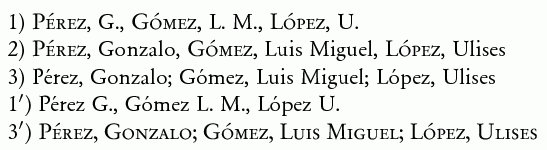
\includegraphics[scale=0.5]{img/eco}
\caption{Nombres en bibliografía}
\end{center}
\end{figure}


En la 1 debe quedar claro que un autor no se identifica por una inicial, por lo que ese dato solo puede corresponder al nombre pospuesto. En la 2 se dan los nombre, pero los apellidos van en versalitas; ya tenemos la diacrisis (es decir, la distinción tipográfica) necesaria y no es necesario ir más allá. En la 3 (y la 3'), en cambio, no hay diferencia alguna entre nombres y apellidos, lo que obliga a separar más claramente los autores con punto y coma. Una variante de la primera es suprimir incluso la coma entre apellido y nombre, en el entendido de que un apellido no puede terminar con unas iniciales. La 3' ha sido muy habitual en España. (Recuérdese que la norma ISO establece que el nombre siempre sigue al apellido.) 

\begin{figure}[h]
\begin{center}
 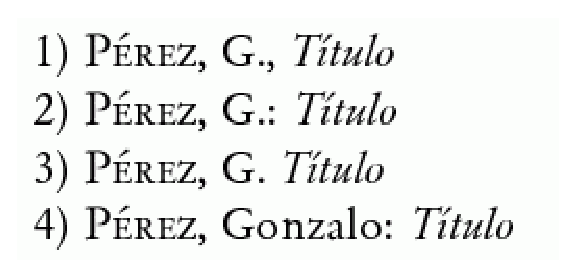
\includegraphics[scale=0.5]{img/eco2}
 \caption{Nombre y título en bibliografia}
\end{center}
\end{figure}

El título siempre debería tener algún tipo de diacrisis, ya sea la cursiva, ya sea el entrecomillado, por lo que los dos puntos son redudantes. La economía en este caso se inclina por la coma. Además, los dos puntos presentan un problema: al ser de la misma altura que las minúsculas e ir pegado a la palabra precedente, se integra visualmente en ella, y en lugar de separar elementos distorsiona uno de ellos (4). La coma, al ser baja, no se integra igual y además crea un espacio adicional que ayuda a distinguir mejor la separación. El punto como separador desaparece tras una inicial (3) pero no tras nombre; en caso de nombres de una letra (que los puede haber) resulta ambiguo y por tanto es mejor evitar este signo. 

\begin{figure}[h]
 \begin{center}
  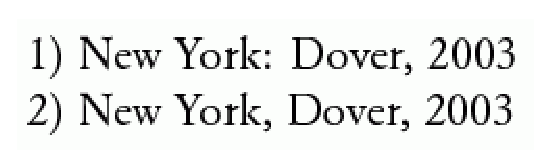
\includegraphics[scale=0.5]{img/eco3}
  \caption{Editorial y año en biliografía}
 \end{center}
\end{figure}

El problema con los dos puntos es el mismo que en el ejemplo anterior. Dado que el orden de los datos es siempre el mismo y la editorial siempre va seguida de la fecha, no tiene por qué darse ninguna ambigüedad en el empleo de la coma, que ha sido la práctica tradicional en español (2): de nuevo la economía diacrítica se inclina por ella. \\



Como en todo, no hay una única manera de hacerlo. Normalmente si se trata de una bibliografía corta y no estamos interesados en reutilizar los datos bibliográficos la elección habitual es escribirla “a mano” mediante el comando \verb|\thebibliography|. Para utilizar datos bibliográficos reutilizables, largos o complejos es preferible emplear la utilidad BibTeX.

El manejo de la bibliografía es semejante al de las referencias, de lo cual ya hemos hablado. En ambos casos, cada registro bibliográfico tiene una etiqueta. Cuando, en una determinada posición del texto, queremos hacer referencia a un registro, hacemos uso del comando \verb|\cite{etiqueta}|. LaTeX ya se encarga de colocar el número o referencia que corresponde a esa entrada y, en el apartado de bibliografía, coloca los datos de la entrada. En caso de que queramos escribir los datos pero no queremos poner una referencia en el texto, utilizamos \verb|\nocite{etiqueta}|.\\

\noindent El entorno \verb|\thebibliography|.



\begin{verbatim}
\begin{thebibliography}{n}
\bibitem{etiqueta}datos
…
\end{thebibliography}
\end{verbatim}

donde etiqueta es la etiqueta que identifica la entrada y datos son los datos de la entrada. Por ejemplo:


\begin{verbatim}
\begin{thebibliography}{9}
\bibitem{Knuth}D. E. Knuth, The TeXbook, Addison Wesley, 1984
\end{thebibliography}
\end{verbatim}


\noindent BibTeX\\

BibTeX es un entorno más complejo para tratar bibliografía, pero es extremadamente útil y fácil de usar. Además, permite reutilizar los ficheros de bibliografía que escribamos para otros
proyectos.

En primer lugar, generamos un fichero al que pondremos un nombre con extensión \verb|.bib|; por ejemplo \verb|mibiblio.bib|. En nuestro caso podría contener lo siguiente:


Tras esta introducción podemos crear un estilo de bibliografía propio siguiendo la norma ISO 690:1987, decir que en \LaTeX{}  ha existido siempre el comando \verb|\bibliography{}| con el que se especifica  uno o más archivos  con extensión .bib que contienen los datos  de las referencias bibliográficas (autor, título, revista, año de edición ...) según un cierto formato.Véase,  como ejemplo:

\begin{verbatim}
 @BOOK{desousa,
  title = {Ortografía y ortotipografía del español actual},
  year = {2004.},
  editor = {Trea},
  author = {José Martínez de Sousa},
  owner = {fcaro},
  timestamp = {2008.08.13}
}
\end{verbatim}

El campo @book nos indica qué tipo de registro es. Hay muchos: para libros, artículos, tesis, manuales, etc. Consulta la documentación de BibTeX para conocerlos. desousa es la etiqueta que identifica el registro que luego citaremos con \verb|\cite|. El resto del archivo está claro qué es. Puede sorprender el uso de {} en el título. Esto se debe a que BibTeX maneja automáticamente las mayúsculas y minúsculas: el la forma de indicarle que no debe modificar lo que va dentro, pues de lo contrario lo pondrá en letras minúsculas.

Es claro que se puede editar a mano una base de datos que siga ese formato sin más que utilizar un editor de texto ASCII, pero hay mejores opciones. Para aquellos quetrabajen en Windows o DOS, recomiendo el programa bibdb, LEd o WinEdt.
Para Linux también hay varias posibilidades para elegir un editor decente como Emacs o Kyle, que en nuestro caso ha sido el elegido y para la creación del archivo \verb|pfcbib.bib.| el cual contiene toda la información de los objetos incluidos en la biliografía hemos utilizado \textbf{JabReF}, que es un gestor de referencias bibliográficas que permite generar bibliografías, Jabref funciona con Java, de manera que es independiente de la plataforma que se esté utilizando, es un editor gráfico de bibliografías para \LaTeX, cuyo formato nativo esta basado en BiB\TeX y que provee una fácil interfaz para utilizar  y editar los archivos de BiB\TeX.

Para su ejecución en Linux JabRef requiere Java VM 1.4.2 o superior para funcionar. En el sitio web del proyecto JabRef, se puede descargar el archivo jabref-*.*.jar. Una vez guardado en el directorio conveniente, se puede ejecutar normalmente desde la consola: 

\begin{verbatim}
 $ java -jar jabref-*.*.jar
\end{verbatim}

\begin{figure}[h]
\begin{center}
 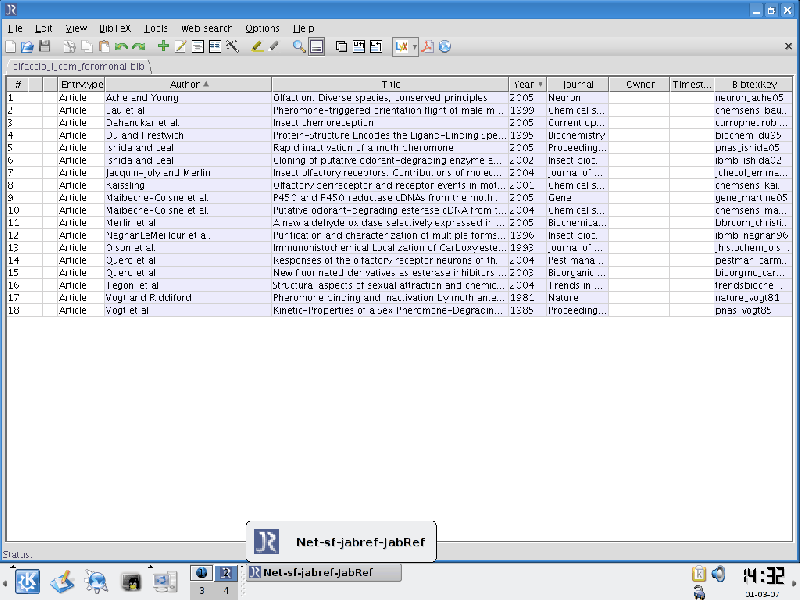
\includegraphics[scale=0.4]{img/jabrefgeneral}
\end{center}
\caption{Vista general interfaz gráfica de JabRef}
\end{figure}


\begin{figure}[h]
\begin{center}
 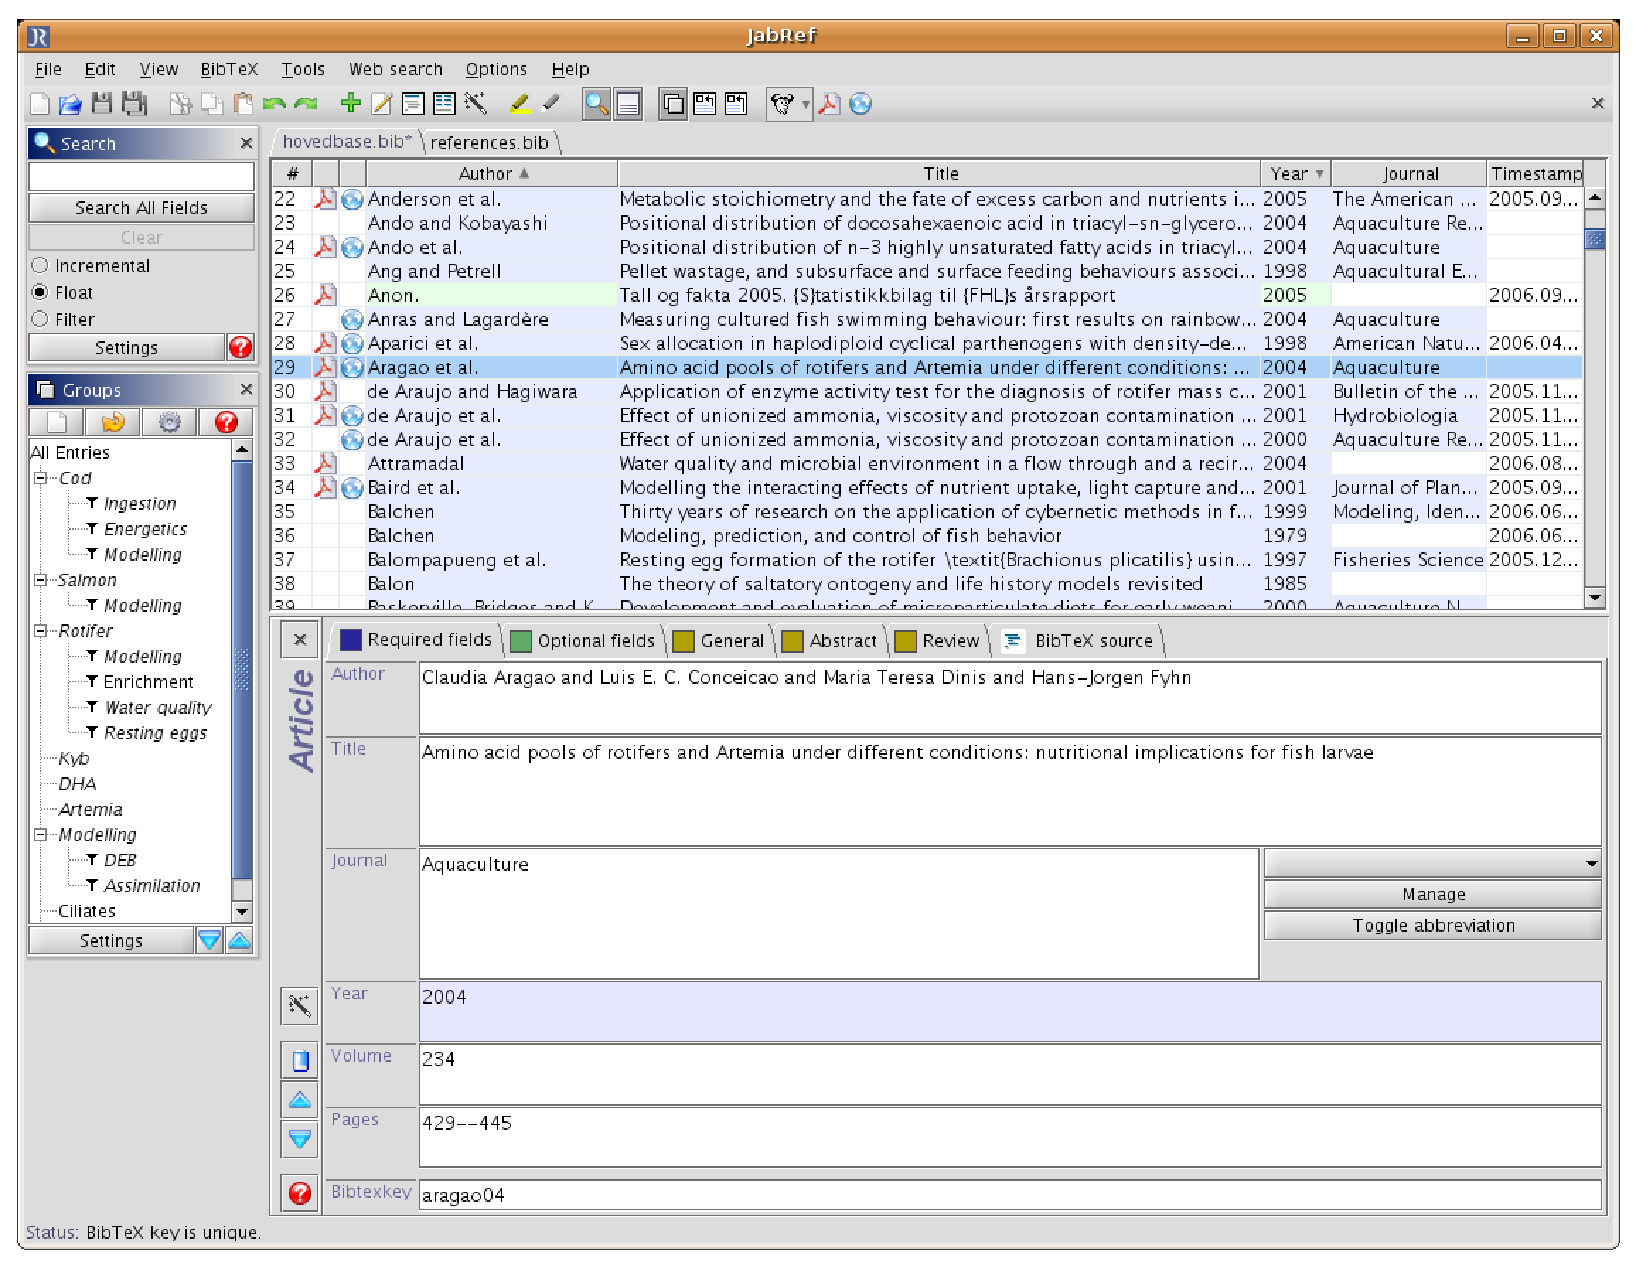
\includegraphics[scale=0.4]{img/jabref}
\end{center}
\caption{Vista de detalle interfaz gráfica de JabRef}
\end{figure}


En el punto de nuestro documento  en el que queremos citar una referencia, incluimos como hemos dicho \verb|\cite{etiquta}|, donde \verb|etiqueta|  ser refiere a la cadena ded caracteres que identifica la referencia deseada dentro del archivo \verb|.bib| que en el ejemplo anterior es \verb|desousa|.Además en el punto en el que se quiera que aparezca, incluimos los comandos \verb|bibliographystyle{estilo.bst}| y \verb|biliography{basededatos.bib}|.El primero se refiere al estilo que se desea utilizar para las referencias, tanto para la anotación que en el texto sustituye al comando \verb|\cite{eiqueta}| como para la ordenación de las referencias y el formato  de cada línea de la lista bibliográfica (esto es, si va el autor, luego el año, luego la revista en cursiva,..).Suelen estar disponibles en todas las instalaciones unos estilos básicos:\verb|plain,alpha,unsrt,abbrv| y hay docenas más para otras necesidades.Conviene saber dónde se guardan por defecto en nuestra instalación de modo que podamos poner otros nuevo en el mismo lugar. Éstas son las únicas adiciones que se deben hacer en el archivo fuente.

A continuación, la primera vez que se pase el archivo fuente por \LaTeX{}, generará un archivo \verb|proyect.aux| que recoge las citas que se hacen a lo largo del documento, así como  el estilo que hemos seleccionado  para la bibliografía  y el nombre  de la base de datos (\verb|pfcbib.bib|).BiB\TeX es un programa externo\footnote{Que se ejecuta con el comando bibtex,fuente.aux aunque depende de cada instalación} que procesa el archivo \verb|fuente.aux| para extraer del \verb|basededatos.bib| los datos de las citas que hayamos incluido y formatearlas según el  estilo seleccionado. Se crea entoces un archivo \verb|fuente.bbl| que contiene un entorno \verb|thebibliogragphy|.La siguiente vez que procesamos el documento,  \LaTeX{}  encuentra el archivo \verb|fuente.bbl| y se incluye ya la bibliografía,  pero normalmente hay que procesar dos veces para que todas las referencias se incluyan correctamente. Como siempre, es interesante prestar atención  a los avisos que se presentan o mirar el archivo \verb|fuente.log| y los que se han ido mencionando para comprobar si todo ha ido bien. Con un poco de suerte, en este punto se acaba el trabajo de incorporar  la bibliografía  a un documento.


\subsubsection{Custom-bib}

Para dar la mayour flexibilidad  en la elección de un estilo para las citas bibliográficas sin necesidad de andar cambiando la base de datos ni hacerse con infinidad de archivos de estilo,Patrick W. Daly, uno de los autores del Kopka y Daly \cite{guidek} ha escrito y mantiene el paquete de macros \verb|custom-bib| que, entre otras cosas, da soporte a distintos idiomas aunque es solo válido para Linux.La última versión 4.1 de 09/08/2003 que se encuentra en la dirección \url{http://www.ctan.org/tex-archive/macros/latex/contrib/custom-bib}.

Un problema que enfrentan los usuarios de BiB\TeX{} es que no existe un estándar para el formato de las listas de referencias. Editoriales y revistas insisten en una colocación de comas completamente arbitraria, dos puntos, y petición de entradas. Por otra parte, el autor (año, estilos de citas cuentan con el apoyo de algunos paquetes especiales \LaTeX{}, pero cada uno de ellos de un número muy limitado de estilos bibliográficos. Por último, la mayoría de esos archivos de estilo son sólo para Inglés, y las adaptaciones a otros idiomas debe duplicar todo el espectro de tales archivos.
	
Todos estos obstáculos son, en principio, fáciles de superar simplemente con una reprogramación de BiB\TeX{} por medio de un archivo de estilo bibliográfico (extensión. BST). BibTEX es de hecho extremadamente flexible, por desgracia, su lenguaje de programación es de muy bajo nivel, permitiendo sólo las más básicas modificaciones para el usuario normal.

La solución a esto es un nombre genérico o el archivo máster de estilo bibliográficos (extension.mbs) que contiene \verb|docstrip| opciones alternativas para la codificación. Al seleccionar las opciones deseadas, se puede personalizar un archivo. BST archivo a su necesidades.

Este archivo, merlin.mbs, es la última versión de uno de propósito general de archivos .mbs para satisfacer la mayor cantidad de necesidades bibliográficas como sea posible. Originalmente fue por Oren Patashnik a partird de archivos estándares tales como  \verb|plain.bst| y \verb|unsrt.bst|, además del archivo no estándar \verb|no-apalike.bst|,  un estilo muy básico autor, año citación estilo. Desde entonces, ha evolucionado ampliamente y se han añadido características que se encuentran a disposición en archivos .bst, y las exigidas por los editores o sugerido muchos usuarios / contribuyentes.

Para utilizarlo este paquete, después de poner todos los archivos que lo componen en algún directorio adecuado, y comprobar que están los archivos \verb|makebst.ins| y varios \verb|mbs|, luego desde la consola de Linux entramos en la carpeta correspondiente a custom-bib y ejecutamos los siguientes comandos:

\begin{verbatim}
 1.	latex makebst.ins

 2.	latex makebst.dtx
\end{verbatim}

El primero crea el archivo \verb|makebst.tex| y el segundo compone el archivo \verb|makebst.dvi| y la documentación de \verb|makebst.pdf| y \verb|merlin.pdf|.Ahora ejecutamos el siguiente comando para que empiece la aplicación.

\begin{verbatim}
 3.	latex makebst.tex
\end{verbatim}

El programa \verb|docstrip|, escrito por Frank Mittelbach, es ahora una parte fundamental de la instalación en \LaTeXe{}.Su objetivo principal es eliminar líneas de comentarios de los archivos documentados, pero tiene la función secundaria de la selección de alternativas de líneas de código.
Un archivo de estilo maestro BiB\TeX{} bibliográficos es uno que, al procesarlo por docstrip con las opciones seleccionadas, produce un archivo Bib\TeX{}.BST con las características deseadas.En este sentido, docstrip funciona  algo así como un preprocesador de C. De hecho, todos los archivos original. BST de Oren Patashnik  se producen a partir de una única fuente de archivos por medio de un preprocesador. La ventaja de \verb|docstrip| es que es portátil a todas las instalaciones con \TeX{}.

	
El programa \verb|docstrip| se puede ejecutar de forma interactiva, donde el usuario debe responder a las preguntas a través del teclado, o por medio de un lote de puestos de trabajo donde todos las entradas se preparan en un archivo de antemano. Para la elaboración de un estilo archivo BiB\TeX{} a partir de un archivo maestro, el método de trabajo en lote (\verb|batch job|) es el único viable, simplemente porque el gran número de opciones disponibles. (Hay otra razón para emplear a un lote de puestos de trabajo: el método interactivo añade un comando \verb|\endinput|  al final, algo sobre lo que  protesta BiB\TeX{}.) El trabajo por lotes en general no tienen ninguna extensión, sino que utiliza  .dbj para \verb|docstrip|. Estos archivos son útiles porque en el documento las opciones usadas para producir el archivo .BST,  y podrán ser modificadas para experimentar con las opciones alternativas.\\


\begin{enumerate}

\item El paquete se ejecuta y empieza a hacer preguntas. Éstas son las primeras preguntas, hay que dar el nombre del archivo de estilo que se va a crear, \verb|pfc| en nuestro caso, la primera pregunta es si queremos un documento de la descripción del uso  del archivo.

\begin{verbatim}
***********************************
* This is Make Bibliography Style *
***********************************
It makes up a docstrip batch job to produce
a customized .bst file for running with BibTeX
Do you want a description of the usage? (NO)

\yn=n
\end{verbatim}

\item A continuación nos pregunta por un archvivo MASTER de base y pondremos \verb|merlin.mbs|.

\begin{verbatim}
Enter the name of the MASTER file (default=merlin.mbs)

\mfile=merlin.mbs
\end{verbatim}

\item Ponemos el nombre del archivo final .bst que obtendremos, pfcbibstyle en nuestro caso.
 
\begin{verbatim}
Name of the final OUTPUT .bst file? (default extension=bst)

\ofile=pfcbibstyle
\end{verbatim}

\item Damos un comentario para incluir en archivo para saber en que ámbito se aplica.
\begin{verbatim}
Give a comment line to include in the style file.
Something like for which journals it is applicable.

\ans=Proyecto Fin de Carrera
\end{verbatim}

\item Si quieres algunos comentarios elocuentes, ponemos que no.
\begin{verbatim}
Do you want verbose comments? (NO)

\yn=n
\end{verbatim}

\item En esta versión de \verb|custom-bib| tenemos el archivo spanish.mbs que nos proporciona la opción de crear el estilo de la bibliografía en español

\begin{verbatim}
 (./merlin.mbs
<<< For more information about the meanings of
<<< the various options, see the section on 
<<< Menu Information in the .mbs file documentation.

EXTERNAL FILES:

Name of language definition file (default=merlin.mbs)

\cfile=spanish.mbs
\end{verbatim}

\item Nos pide si incluimos archivos para los nombres de diarios extras, decimos que no.

\begin{verbatim}
 Include file(s) for extra journal names? (NO)

\yn=n
\end{verbatim}

\item Seleccionamos el estilo para las citaciones, en nuestro caso \verb|Alpha style| con opción de varios autores,  opcion (b).

\begin{verbatim}
 STYLE OF CITATIONS:
(*) Numerical as in standard LaTeX
(a) Author-year with some non-standard interface
(b) Alpha style, Jon90 or JWB90 for single or multiple authors
(o) Alpha style, Jon90 even for multiple authors
(f) Alpha style, Jones90 (full name of first author)
(c) Cite key (special for listing contents of bib file)
  Select:

\ans=b
\end{verbatim}

\item Para la salida de código HTML seleccionamos  normal de \LaTeX{}, opción (*).

\begin{verbatim}
 HTML OUTPUT (if non author-year citations)
(*) Normal LaTeX output
(h) Hypertext output, in HTML code, in paragraphs
(n) Hypertext list with sequence numbers
(k) Hypertext with keys for viewing databases
  Select:

\ans=*
\end{verbatim}

\item Para esta pregunta seleccionamos la opción (*).

\begin{verbatim}
LANGUAGE FIELD
(*) No language field 
(l) Add language field to switch 
    hyphenation patterns temporarily
  Select:
\ans=* 
\end{verbatim}

\item Seleccionamos que no queremos anotaciones, opción (*).

\begin{verbatim}
 ANNOTATIONS:
(*) No annotations will be recognized
(a) Annotations in annote field or in .tex 
    file of citekey name
  Select: 
\ans=*
\end{verbatim}

\item No tenemos presentaciones luego seleccionamos opción (*).

\begin{verbatim}
PRESENTATIONS:
(*) Do not add presentation type for conference talks
(p) Add presentation, speaker not highlighted 
(b) Presentation, speaker bold face 
(i) Presentaion, speaker italic 
(c) Presentaion, speaker in small caps 
  Select:

\ans=*
\end{verbatim}

\item Seleccionamos ordenación por apellido principal, opción (x).

\begin{verbatim}
 ORDER ON VON PART (if not citation order)
(*) Sort on von part (de la Maire before Defoe)
(x) Sort without von part (de la Maire after Mahone)
  Select:

\ans=x
\end{verbatim}

\item Para la forma en que aparecen los nombres de los autores seleccionamos apellido, nombre completo, opción (f).

\begin{verbatim}
 AUTHOR NAMES:
(*) Full, surname last (John Frederick Smith)
(f) Full, surname first (Smith, John Frederick)
(i) Initials + surname (J. F. Smith)
(r) Surname + initials (Smith, J. F.)
(s) Surname + dotless initials (Smith J F)
(w) Surname + comma + spaceless initials (Smith, J.F.)
(x) Surname + pure initials (Smith JF)
(y) Surname + comma + pure initials (Smith, JF)
(z) Surname + spaceless initials (Smith J.F.)
(a) Only first name reversed, initials 
    (AGU style: Smith, J. F., H. K. Jones)
(b) First name reversed, with full names 
    (Smith, John Fred, Harry Kab Jones)
  Select:
\ans=f
\end{verbatim}
\item  Los nombres de los editores  los dejamos normal, opción (*).

\begin{verbatim}
 EDITOR NAMES IN COLLECTIONS (if author names reversed)
(*) Editor names NOT reversed as edited by John James Smith
(r) Editor names reversed just like authors'
  Select:

\ans=*
\end{verbatim}

\item Posición de Junior, opción (*).

\begin{verbatim}
 POSITION OF JUNIOR (if author names reversed)
(*) Junior comes last as Smith, John, Jr.
(m) Junior between as Smith, Jr., John
  Select:

\ans=*
\end{verbatim}

\item Elegimos el punto y coma para separar los nombre de los autores, opción (s).

\begin{verbatim}
 PUNCTUATION BETWEEN AUTHOR NAMES:
(*) Author names separated by commas 
(s) Names separated by semi-colon 
(h) Names separated by slash /
  Select:

\ans=s
\end{verbatim}

\item Referencias adyacentes con nombres repetidos siempre presentes, opción (*).

\begin{verbatim}
 ADJACENT REFERENCES WITH REPEATED NAMES:
(*) Author/editor names always present 
(d) Repeated author/editor names replaced by dash 
(2) Repeated author/editor names replaced by 2 dashes 
(3) Repeated author/editor names replaced by 3 dashes 
  Select:

\ans=*

\end{verbatim}

\item Número de autores en la biliografía,  los ponemos todos, opción (*).

\begin{verbatim}
 NUMBER OF AUTHORS IN BIBLIOGRAPHY:
(*) All authors included in listing
(l) Limited authors (et al replaces missing names)
  Select:

\ans=*
\end{verbatim}

\item Autores en citaciones, opción (*)

\begin{verbatim}
 AUTHORS IN CITATIONS:
(*) One author et al for three or more authors
(m) Some other truncation scheme 
  Select:

\ans=*

\end{verbatim}

\item Tipo de fuente para las referencias de nombres de los autores, opción (*).

\begin{verbatim}
 TYPEFACE FOR AUTHORS IN LIST OF REFERENCES:
(*) Normal font for author names 
(s) Small caps authors (\sc)
(i) Italic authors (\it or \em)
(b) Bold authors (\bf)
(u) User defined author font (\bibnamefont)
  Select:

\ans=*
\end{verbatim}

\item Posición de la fecha al final de todo, opción (e).

\begin{verbatim}
 DATE POSITION:
(*) Date at end 
(b) Date after authors 
(j) Date part of journal spec. (as 1994;45:34-40) else at end
(e) Date at very end after any notes
  Select:

\ans=e
\end{verbatim}

\item Formato de la fecha precedido de coma, opción (m).

\begin{verbatim}
 DATE FORMAT (if non author-year citations)
(*) Plain month and year without any brackets
(p) Date in parentheses as (May 1993)
(b) Date in brackets as [May 1993]
(c) Date preceded by colon as `: May 1993'
(d) Date preceded by period as `. May 1993'
(m) Date preceded by comma as `, May 1993'
(s) Date preceded by space only, as ` May 1993'
  Select:

\ans=m

\end{verbatim}

\item Solo pondremos en la fecha el año sin el mes, opción (x).

\begin{verbatim}
 SUPPRESS MONTH:
(*) Date is month and year 
(x) Date is year only 
  Select:

\ans=x
\end{verbatim}

\item Tipo de fuente normal para la fecha,  opción (*).

\begin{verbatim}
 DATE FONT:
(*) Date in normal font 
(b) Date in bold face 
  Select:

\ans=*
\end{verbatim}

\item El título debe de tener diacrisis por lo tanto opción (i).

\begin{verbatim}
 TITLE OF ARTICLE:
(*) Title plain with no special font
(i) Title italic (\em)
(q) Title and punctuation in single quotes (`Title,' ..)
(d) Title and punctuation in double quotes (``Title,'' ..)
(g) Title and punctuation in guillemets (<<Title,>> ..)
(x) Title in single quotes (`Title', ..)
(y) Title in double quotes (``Title'', ..)
(z) Title in guillemets (<<Title>>, ..)
  Select:

\ans=i
\end{verbatim}



\item Opción (*).

Sigue haciendo preguntas hasta esta última:
.
\begin{verbatim}

Finished!!
Batch job written to file `pfcbibstyle.dbj'
Shall I now run this batch job? (NO)

\yn=y
\end{verbatim}
Después de responder a todas estas preguntas obtendremos el archivo pfcbibstyle.bst en la carpeta  custom-bib.








\end{enumerate}




\pagebreak

	
\section{Macros}\label{macro}
Según el texto sacado de \cite{valiente}, dado que \LaTeX{} es un sistema de marcado, todo documento \LaTeX{} contiene una serie de \emph{marcas}, o \emph{macros} como las llamaremos a partir de ahora, dentro del texto mismo del documento.Estas \emph{macros} permiten especificar gran variedad de aspectos que definene la forma de presentación del documento, desde consideraciones ortográficas y tipográficas sencillas de las que hablaremos en la sección \ref{sec:ortotip} hasta la estructura del documento.
Prácticamente todas las \emph{macros} del sistema \LaTeX{} se escriben con caracteres ASCII y comienzan con un barra invertida \verb|"\"|. Hay cerca de un millar de \emph{macros} estándar pero cada autor de \LaTeX{} puede definir nuevas \emph{macros}.Por ejemplo la \emph{macro} estándar \verb|\textbf{|\emph{texto}\verb|}| compone su argumento \emph{texto} en \textbf{negrita}.Uno de los usos de negrita podría ser para resaltar una palabra. Entonces el autor puede definir una nueva \emph{macro}, \verb|resaltar|, que produce el mismo efecto que la macro \verb|\textbf{}|.
La definición de la nueva macro \verb|resaltar| se hace mediante una macro estándar de \LaTeX, \verb|\newcommand|: \\

\verb|\newcommand{\resaltar}[1]{\textbf{#1}}| \\

donde \verb|[1]| indice que la macro \verb|\resaltar{}| tiene un argumento y \verb|\textbf{#1}| indica que el argumento número 1 o primero (y en este caso único) \verb|#1| se ha de componer con negrita. Una vez hecha esta definición, se puede escribir \verb|\resaltar{palabra}| dentro del texto del documento para  obtener \textbf{negrita} como resultado.

La ventaja de introducir nuevas \emph{macros} dentro de un documento \LaTeX{} es que éstas permiten  definir nombres más comprensibles para el autor, pero también modificar  de una manera fácil y rápida  el efecto de una misma macro en todo el documento \LaTeX{}. Por ejemplo si se quiere hacer que la \emph{macro} resaltar en vez de hacer \textbf{negrita} se haga resaltar las palabras con \emph{cursiva} solo hay que poner:\\

\verb|\newcommand{\resaltar}[1]{\emph{#1}}| \\

Es por esto por lo que es muy importante definir en el preámbulo del documento \LaTeX{} las \emph{macros} para los efectos tipográficos que se han de aplicar en el texto del documento, incluso cuando éstas no son nada más que sinónimos de otras \emph{macros} estándares de \LaTeX{}:\\
La forma general de hacer:\\

\verb|\newcommand{\macro}[n]{definición}| \\

donde \emph{n} es el número de argumentos o parámetros de la macro (9 como máximo) y \emph{definición} puede usar los \emph{n} parámetros \verb|#1,#2,#3,.....,#n.|

La activación de un \emph{macro}  en \verb|newcommand| da un error en \LaTeX{} si la macro que se define ya había sido definida, o si se trata de una de las \emph{macros} predefinidas por \LaTeX{}.En estos casos es posible modificar la definición de la macro existente mediante la \emph{macro}:\\

\verb|renewcommand| \\

\noindent En general, sin embargo, no es aconsejable cambiar la definición de una \emph{macro} predefinida de \LaTeX{} salvo que se conozca su funcionalidad con todo detalle y que se sepa exactamente qué uso se ha hecho  en el documento \LaTeX{} y también que uso se quiere hacer.Resulta conveniente entonces cambiar el nombre de la macro por otro que todavia no haya sido utilizado.

Las \emph{macros} de \LaTeX{} pueden afectar a la totalidad el texto del documento como a un párrafo o incluso palabra  o carácter.Así se necesita un mecanismo para indicar el ámbito de actuación de cada macro introducida en el documento.

El mecanismo básico para indicar el ámbito de una  \emph{macro}  es la agrupación entre llaves :\verb|{texto}| .Por ejemplo la macro \verb|\emph| sirve para dar énfasis en un parte relativamente pequeña del documento, tal como unas pocas palabras componiéndolas con letras cursivas si sus letras son redondas y componiéndolas con letras redondas si su texto es cursivo.Así \verb| \emph palabra| da énfasis al primer carácter de \emph palabra mientras que  \verb|emph{palabra}| produce \emph{palabra}.

Otro mecanismo para indicar el ámbito de \emph{macros} es el uso de \emph{macros} de inicio y fin, los llamados entornos de \LaTeX{}. Por ejemplo, \verb|begin{center}| \emph{párrafo} \verb|\end{center}|  es un entorno que permite alinear horizontalmente el texto del párrafo incluido en el entorno.

Finalmente hay ciertas \emph{macros} de \LaTeX{}, llamadas \emph{declaraciones} que tienen un efecto global en el documento, como por ejemplo \verb|\em|, a pesar que su efecto es local si se incluyen dentro de un grupo de llaves o de un entorno.

Toda declaración tiene asociado un entorno correspondiente, el cual lleva el mismo nombre que la declaración pero sin la barra invertida, asi la declaración :\\

\verb|{\em texto}|\\

\noindent es equivalente al entorno\\

\verb|\begin{em}|\emph{texto}\verb|\end{em}| \\

El hecho de escribir entornos en lugar de declaraciones puede dar como resultado un original más fácil de leer,  sobre todo cuando el texto de la declaración es bastante largo, ya que suele ser más fácil encontra los delimitadores de un entorno que las llaves que delimitan el ámbito de una declaración.

\subsection{Macros de la clase}

Con el objetivo de facilitar diversas tareas al usuario de esta clase, hemos definido en ella una serie de macros con diferentes funcionalidades. En este apartado veremos con detalle dichas macros y sus posibles utilidades.

Para comenzar tenemos definiciones sencillas para facilitar la escritura en \LaTeX. Se utilizan para faciliatar a la hora de escribir palabras reservadas como \verb|\LaTeX{}|, que sería los mismo que poner \verb|latex|.Se podría hacer lo mismo con cualquier otra palabra o frase.
\codigofuente{TeX}{Macros sobre \LaTeX{}}{codigo/macrotex}

Para hacer la inserción de archivos de código fuente en múltiples lenguajes de programación según el cuadro \ref{tab:lenglist},hemos definido la siguiente macro que tiene tres variables de entrada cuyo funcionamiento podemos ver en la imagen.
\codigofuente{TeX}{Macro para código fuente}{codigo/macrocodfuente} 

\LaTeX{} tiene muchas formas de incluir imágenes, para ello es necesario hacer uso del paquete:

\noindent \verb|\usepackage{graphicx}| 

\noindent y el comando:

\noindent \verb|\includegraphics[opciones]{nombre}|

Según las necesidades se pueden insertar las imágenes en cualquier parte del documento incluso rodeado por texto, imágenes invertidas y otras muchas opciones que se pueden encontrar en cualquier manual. La siguiente macro contiene el posicionamiento y las opciones básicas de inserción de imágenes, es decir en el centro del documento, arriba o abajo según convega, una referencia y una etiqueta. Para todas estas opciones la macro tiene cinco variables de entrada cuyo funcionamiento podemos ver a continuación.

\codigofuente{TeX}{Macro para insertar imágenes}{codigo/macrofigura}

Los cuadros en \LaTeX{} al igual que las figuras tiene muchísimas opciones, en nuestro caso la macro crea una tabla sencilla en la que podemos especificar el número de columnas y filas, el título de el cuadro y la etiqueta, tiene cuatro variables de entrada cuyo funcionamiento podemos ver a continuación.
 
\codigofuente{TeX}{Macro para insertar cuadros}{codigo/macrotabla}

Para la portada hemos creado macros para los datos de entrada que necesita la el comando \verb|\hacerportada|. Hemos creado macros para autores, titulación, título, tutor y departamento.El código es el siguiente:

\codigofuente{TeX}{Macros para variables de portada}{codigo/macroclsdatoportada}

\section{Entornos}

Para más facilidad a la hora de utilizar el paquete \verb|amsthm| hemos creado nuevos entornos con la traducción a español con el siguiente código:

\codigofuente{TeX}{Entorno para amsthm}{codigo/codigoamsthm}

También hemos creado un entorno para crear un cuadro como el utilizado en el capítulo \ref{errores}, el código para su creación lo vemos a continuación:

\codigofuente{TeX}{Entorno para cuadro vacío}{codigo/codigocuadrovacio}












\section{Ortotipografía}\label{sec:ortotip}

La \textbf{ortotipografía} es el conjunto de usos y convenciones particulares con las que se rige la escritura por medio de elementos tipográficos en cada lengua. Se ocupa de la combinación de la ortografía y la tipografía y en particular la forma en que la primera se aplica en las obras impresas.

Martínez de Sousa \cite{desousa} define la ortotipografía como «el conjunto de reglas de estética y escritura tipográfica que se aplican a la presentación de los elementos gráficos», como las bibliografías, cuadros, poesías, índices, notas de pie de página, citas, citas bibliográficas, obras teatrales, aplicación de los distintos estilos de letra (redonda, cursiva, versalitas, así como las combinaciones de unas y otras), etc.

Para aclarar más sobre ortografía, tipografía y ortotipografía,  en qué consisten, para qué sirven y en qué se diferencian, tenemos una breve introducción de Javier Bezos en la web \url{http://www.tex-tipografia.com/ortotypo.html} y de la que hemos extraido este texto.\\

La \textbf{ortografía} es el conjunto de normas que regulan la escritura de una lengua. La ortografía decide, por ejemplo, qué letras concretas han de emplearse para escribir una palabra (como \textit{v} o \textit{b}, \textit{g} o \textit{j}...), cuándo se emplean mayúsculas, el significado básico de signos como la coma, las comillas, etc. La ortografía se aplica a todo tipo de escritos, ya sean tipográficos o caligráficos.\\

La \textbf{tipografía} es el arte de crear y combinar tipos, es decir, letras de imprenta, para producir libros, revistas, folletos, etc., con el objetivo de facilitar su lectura y que el contenido se transmita de forma eficaz.\\

La \textbf{ortotipografía} (en inglés \textit{typographical syntax}) estudia la combinación de la ortografía y la tipografía y concreta la forma en que la primera se aplica en obras impresas. Un par de ejemplos pueden ser ilustrativos: \\
\begin{itemize}
\item la ortografía establece que las siglas han de escribirse con mayúsculas, pero un tipógrafo observará que su mayor tamaño produce «manchas» en la página que pueden distraer al lector y por tanto se introduce la norma ortotipográfica de que esas mayúsculas se pueden componer como versalitas o a un tamaño menor;
\item  el punto cierra oraciones, pero si coincide con una llamada de nota voladita, se pueden producir «escalones» visuales que, de nuevo, pueden distraer al lector, por lo se desplazan las llamadas para que sigan al punto.
\end{itemize}

\subsection{Ortotipografía de programas informáticos}
También en la web de Javier Bezos hay disponible una publicación sobre ortotipografía informática que se encuentra en su Versión 0.1. 2007-03-14 la cual tenemos a continuación:\\

  Este documento tiene como propósito proporcionar una serie de reglas generales
sobre la composición de código informático destinado a técnicos, autores, editores
y correctores que tienen que tratar con obras o artículos de este tipo.\\

\noindent\textbf{Código}

  El código escrito en algún lenguaje de programación deberá distinguirse tipográ-
ficamente del texto, normalmente con letra sin remates o mecanográfica.\\

\noindent\textbf{Listados de código}

  En los bloques de código que ocupan varias líneas, se deberá prestar atención a
la posibilidad de que la medida del texto sea inferior a la longitud de las líneas del
código. Es ese caso, no se dejará que el código pase simplemente a la línea siguiente
(y menos sin sangrar), sino que se organizará siguiendo las reglas sintácticas del
lenguage, normalmente con sangrado adicional, y en ocasiones con el apoyo de
algún signo especial (ninguno en C, Java o Pascal, pero \verb|\| en Python, \verb|_| en Visual
Basic y $\neg$ AppleScript, por ejemplo).\\

\begin{verbatim}
 if (png_info (img)->valid & PNG_INFO_pHYs) {
    img_xres (img) = round (0.0254 *
        png_get_x_pixels(png_ptr (img), png_info (img)));
    img_yres (img) = round (0.0254 *
        png_get_y_pixels(png_ptr (img), png_info (img)));
}
\end{verbatim}

y no

\begin{verbatim}
 if (png_info (img)->valid & PNG_INFO_pHYs) {
    img_xres (img) = round (0.0254 *
png_get_x_pixels_per_meter (png_ptr (img), png_info (img)));
    img_yres (img) = round (0.0254 *
png_get_y_pixels_per_meter (png_ptr (img), png_info (img)));
}
\end{verbatim}

 También se puede emplear un signo especial que indique que una línea es conti-
nuación de la anterior y que debe considerarse que en el código es en realidad una
sola línea:\\


\noindent\verb|if (png_info (img)->valid & PNG_INFO_pHYs) {|\\
    \indent\verb|img_xres (img) = round (0.0254 *|\\
	\indent\indent\ArrowBoldDownRight  \verb|png_get_x_pixels(png_ptr (img), png_info (img)));|\\
    \indent\verb|img_yres (img) = round (0.0254 *|\\
	\indent\indent\ArrowBoldDownRight  \verb|png_get_y_pixels(png_ptr (img), png_info (img)));|\\
\verb|}|\\

\noindent\textbf{Alineación}

Cuando la letra sea mecanográfica, se ajustarán las líneas de forma que los caracteres
resulten alineados verticalmente, por lo que el espacio ha de ser fijo:
\begin{verbatim}
for f in fndf.split(’\n’):
    f = f.strip()
end
\end{verbatim}
y no
\begin{verbatim}
for f in fndf.split(’\n’):
     f = f.strip()
end
\end{verbatim}


\noindent\textbf{Código en texto}

Contra la norma general, los signos de puntuación pegados al código pero que no
forman parte de él, deben ser de la letra principal, aunque conservando la figura y el
trazo. Además, los espacios del código, incluso si forman parte de él, deben ser los
que corresponden al texto (en la letra mecanográfica suelen ser fijos y más anchos,
lo que resta uniformidad a los párrafos).\\

\small Entre los métodos de la clase \texttt{String} están: \textbf{\textit{count, find, index, join, split, strip}}
\indent y otros\\

\indent\indent y no\\

Entre los métodos de la clase \texttt{String} están: \textbf{\textit{count, find, index, join, split, strip}}
\indent y otros.\\

La orden \verb|a.put(x, i)| asigna x al valor i-ésimo de \verb|a.|\\


\indent\indent y no\\

La orden \verb|a.put (x, i)| asigna x al valor i-ésimo de \verb|a.|\\

\normalsize
\noindent\textbf{Puntuación}

Los listados de código, es decir, el código que no está en el texto sino dispuesto
aparte, no llevarán ningún signo de puntuación que no les corresponda, incluso si
les pudiera corresponder por su posición en el texto (coma, punto, etc.). Si se trata
de un código breve del texto, que cita una orden, la explica, etc., sí se pondrá la
puntuación que corresponde al texto.\\

\noindent\textbf{Licencia}

Este documento se puede distribuir e imprimir libre y gratuitamente tanto en formato
electrónico como impreso, pero su contenido está bajo \textit{copyright} del autor y no
se puede copiar, ni reproducir en otras obras sin autorización previa del autor, salvo
en caso de cita tal y como prevé la legislación española.
\copyright 2005-2007. Javier Bezos.

